\chapter{The Standard Model of Particle Physics}\label{ch:sm}
\noindent The \ac{sm} of Particle Physics is the current theory that describes three of the four fundamental forces, namely the electromagnetic, strong, and weak forces, with the exception of gravity. Over the last decades it has been probed with remarkable precision. However, as discussed later in this chapter, there are still observational phenomena that lie beyond its scope.

The \ac{sm} is based on symmetry principles and is described by a lorentz-invariant \ac{qft} that is renormalizable and invariant under local gauge transformations. This means that within the non-abelian gauge group
\begin{equation}
    G = SU(3)_C \otimes SU(2)_L \otimes U(1)_Y,
\end{equation}
the equations of motions remain invariant. $SU(3)_C$ is the special unitary group of rank 3 representing the color symmetry within \ac{qcd}, the \ac{qft} describing the strong interactions. $SU(2)_L \otimes U(1)_Y$ exhibits the unification of the weak and electromagnetic interaction into the \ac{ew} force of $SU(2)_L$ left-chiral fermions of the weak force and right-handed $U(1)_Y$ fermions with weak hypercharge $Y$ of the electromagnetic force described by \ac{qed}.

The following describes the particles of the \ac{sm} and gives a brief overview of the \ac{qft}'s used to describe aforementioned forces. The content of this chapter draws inspiration primarily from \citep{hollik2010quantum,griffiths2020introduction,thomson2013modern,zee2010quantum,halzen1984introductory}. Natural units are assumed everywhere $\hbar=c=1$.


\section{Particles of the Standard Model}

All currently known elementary particles are included in the \ac{sm} and can be organized as depicted in figure \ref{fig:sm}. This includes 12 fermions, that are particles of half-integer spin, 12 vector bosons with spin 1, and the Higgs boson, a scalar particle with spin 0.


\begin{figure}
    \centering
    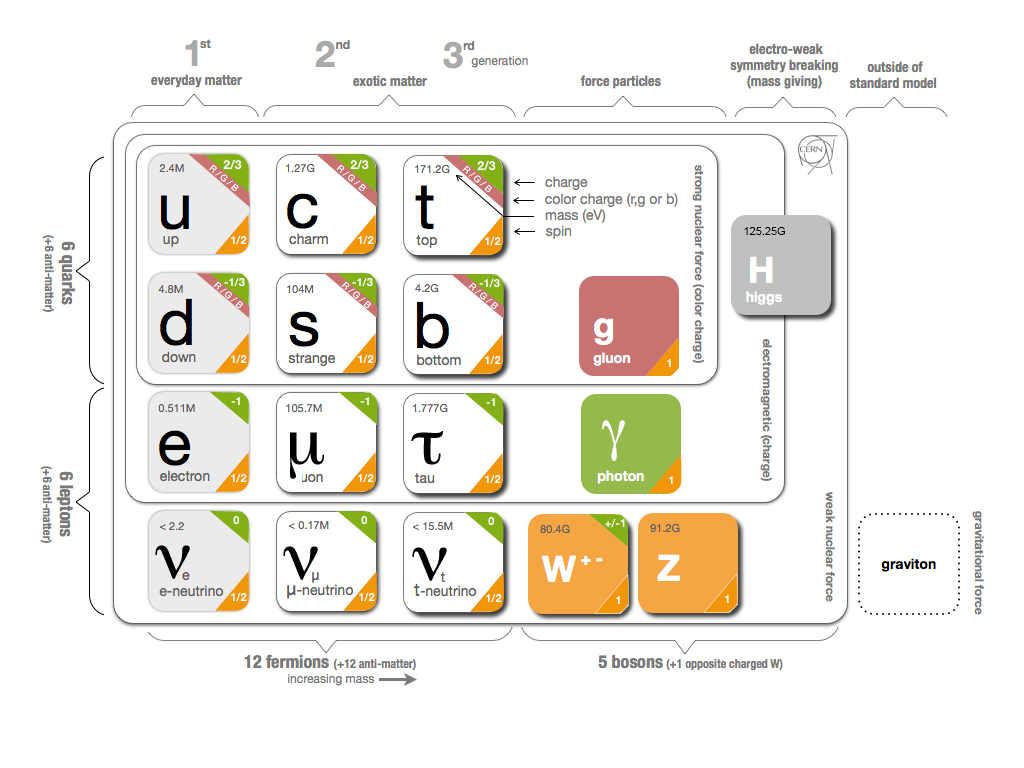
\includegraphics[width=1\textwidth]{SMinfographic_image_}
    \caption[]{Particles in the SM. Adopted from \citep{smpar}. Higgs Boson mass corrected to the current value \citep{particle2022review}. }
    \label{fig:sm}
\end{figure}


The fermions can be categorized into three generations each consisting of a charged lepton, a neutral neutrino and two quarks. Except for their masses, particles of different generations have the same quantum numbers. Ordinary matter consists only of particles from the first generation. Moreover each particle has an associated anti-particle with all the quantum numbers inversed.

Quarks possess both electric charges and color charges, causing them to interact with each other via weak, electromagnetic, and strong forces. Each generation consists of an up quark (up, charm and top quark) with an electric charge of \mbox{Q = 2/3} and a down quark (down, strange and bottom quark) with a charge of \mbox{Q = -1/3}. Due to color confinement, quarks can only be observed as composite particles called hadrons. This principle states that attempting to separate a hadron always results in the production of a quark-antiquark pair due to energetic favorability. Hadrons are either bound states of two quarks (mesons, e.g., a pion) or three quarks (baryons, e.g., a proton). To comply with Pauli's exclusion principle, quarks in a bound state must have different color states.

Leptons in turn do not carry a color charge and encompasses the electron $e$, muon $\mu$ and tau $\tau$ and their associated neutrinos $\nu_e$, $\nu_\mu$ and $\nu_\tau$. In the \ac{sm} neutrinos are considered to be massless. Neutrinos also do not carry a charge and interact solely via the weak force whereas the ones ($e$, $\mu$, $\tau$) with a charge $Q=-1$ also interact electromagnetically.

In the interaction picture of \ac{qft}, forces are mediated by particles specific to the particular force. These particles are bosons and are mediating as 8 massless gluons $g$ the strong force, as 1 massless photon $\gamma$ the electromagnetic force and as 3 massive bosons $W^+,W^-,Z$ the weak force.

The scalar Higgs particle has a unique role in the Standard model. A locally gauge invariant \ac{qft} requires massless mediators, which the $W^{\pm},Z$ are not. When unifying the weak force and the electromagnetic force into the electroweak force a new field - the Higgs field - incorporates mass to these mediators by leaving the \ac{qft} gauge invariant. This will be discussed in detail in section \ref{sec:higgs_mechanism}. The Higgs field can also explain the masses of all fermions as the coupling to each fermion is proportional to its mass. This essentially means that the heavier the particle, the stronger its interaction is with the Higgs field.

If not further specified the following always includes the anti-particles when referred to a species or a particular particle.

\section{Elements of Quantum Field Theory}\label{sec:qft}
Elementary particles can be created, transformed, and annihilated in various forms of particle interactions. These phenomena can be understood through special relativity and quantum mechanics. Special relativity relates energy with mass, allowing energy to manifest as massive particles. Quantum mechanics, through the uncertainty principle, states that energy can fluctuate significantly over short time scales.

However, special relativity lacks a quantum mechanical description, and in non-relativistic quantum mechanics, the particle number is conserved. \ac{qft} was developed to provides a solution to this dilemma and to incorporate observations into a unified theory.

For a field description, some quantity $\phi(x,y,z,t)=\phi(x)$ is assigned to some region in spacetime $x$. Similar to the Lagrangian formalism in classical mechanics here a Lagrangian density in spacetime governs the dynamics of the system $\mathcal{L}(\phi_1,\dots,\phi_n) =T-V$.
    {\renewcommand{\arraystretch}{1.7} %<- modify value to suit your needs
        \begin{table}
            \begin{center}
                \begin{tabular}{c|c|c}
                    particle           & field type      & Lagrange                                                                                                     \\ \hline
                    spin-0 (scalar)    & scalar $\phi$   & $\mathcal{L}_\mathrm{Klein-Gordon}=\frac{1}{2} (\partial_\mu \phi )(\partial^\mu \phi)-\frac{m^2}{2}\phi^2 $ \\
                    spin-1/2 (fermion) & spinor $\psi$   & $\mathcal{L}_\mathrm{Dirac}= \overline{\psi}(i \gamma^\mu \partial_\mu - m )\psi$                            \\
                    spin-1 (boson)     & vector  $A_\mu$ & $\mathcal{L}_\mathrm{Proca}= -\frac{1}{4}F_{\mu\nu}F^{\mu\nu} +\frac{m^2}{2} A_\mu A^\mu$                    \\ [.7ex]
                \end{tabular}
                \caption{Quantum fields relevant for the \ac{sm}. With $F_{\mu\nu}=\partial_\mu A_\nu - \partial_\nu A_\mu$ the electromagnetic field strength tensor.}
                \label{tab:fields}
            \end{center}
        \end{table}
    }
Fields which appear in the \ac{sm} and their associated Lagrangian are summarized in table \ref{tab:fields}.
% Via the generalized Euler-Lagrange equations of \ac{qft} 
% \begin{equation}
%     \partial_\mu \left(\frac{\partial\mathcal{L}}{\partial(\partial_\mu\phi_i)}\right)=\frac{\partial\mathcal{L}}{\partial \phi_i}.
% \end{equation}
% the according equations of motion associated with the fields can be obtained.

In \ac{qft} the conventional strategy to describe particle dynamics is to use a perturbation ansatz $\mathcal{L}=\mathcal{L}_0+\mathcal{L}_1$ where one knows the solution of $\mathcal{L}_0$ and adds a small perturbation $\mathcal{L}_1$ so that $\mathcal{L}$ can be solved \citep{zee2010quantum}. Here the free field/kinetic part of the Lagrangian is \mbox{$\mathcal{L}_0=\frac{1}{2}[(\partial_\mu \phi)^2 - m^2\phi^2] $} and a small perturbation/potential term $\mathcal{L}_1=V(\phi)$ is added as some polyominal in $\phi$ that governs the interactions of particles. A term $J(x)\phi(x)$ needs to be added to excite the field or create/destroy particles so that the ansatz reads
\begin{equation}
    \mathcal{L}=\frac{1}{2}[(\partial_\mu \phi)^2 - m^2\phi^2]
    -V(\phi) + J(x)\phi(x).
\end{equation}
In the path integral formulation of \ac{qft} the problem can be reduced to integrals of the form \mbox{$\int D\phi e^{i\int d^4x \mathcal{L}(\phi(\bm{x},t))}$}. Where $\int D\phi$ is the integral over all possible paths of the field. Usually the perturbation $V(\phi)$ is just one anharmonic term with $\lambda\phi^4$ with coupling strength $\lambda$ and is expanded in $e$ to make the integral solvable
\begin{equation}
    e^{-V(\phi)}=e^{-\lambda\phi^4}=1-\lambda\phi^4+\frac{1}{2}\lambda^2\phi^8+\dots
\end{equation}
This only works if $\lambda$ is small. With this the Lagrangian can be solved and the result is a probability also called the amplitude usually denoted with $\mathcal{M}$. Via this one can derive the Feynman rules and calculate cross-sections to a desired order of expansion.

The forces and Lagrangians occurring in the \ac{sm} are discussed in the following sections on \ac{qed} \ref{sec:qed}, \ac{qcd} \ref{sec:qcd} and the \ac{ew} theory \ref{sec:ew}. For these the principle of local gauge invariance plays a key role and is inspired by gauge invariance from classical electrodynamics.

\section{Quantum Electrodynamics}\label{sec:qed}
The \ac{qft}-description of the electromagnetic interaction \ac{qed} can be derived from the free fermion field given by the Dirac equation
\begin{equation}
    \mathcal{L}_\mathrm{Dirac} = \overline{\psi}(i \gamma^\mu \partial_\mu - m )\psi.
    \label{eq:dirac}
\end{equation}
This Lagrangian is invariant, i.e. the equations of motion remain unchanged, under a change of a phase $\alpha$
\begin{equation}
    \psi(x) \rightarrow  e^{-i \alpha}\psi(x).
\end{equation}
The requirement that this transformation also holds locally means that $\alpha$ now additionally depends on the point $x$ in spacetime $\alpha \rightarrow \alpha(x)$. Since this gives another term because of the derivative, the Lagrangian can be made invariant again by introducing a vector field $A_\mu$ with a coupling of the size of the electron charge $e$ and replacing the derivative $\partial_\mu$ by the covariant derivative $D_\mu$
\begin{equation}
    \partial_\mu \rightarrow D_\mu = \partial_\mu + ie A_\mu.
    \label{eq:cov_diff}
\end{equation}
Thus, the new Lagrangian
\begin{equation}
    \mathcal{L} = \overline{\psi}(i \gamma^\mu D_\mu - m )\psi
    =
    \underbrace{\overline{\psi}(i \gamma^\mu \partial_\mu - m )\psi}_{\mathcal{L}_\mathrm{Dirac} }
    +
    \underbrace{ e\overline{\psi} \gamma^\mu {\psi}A_\mu}_{\mathcal{L}_\mathrm{int}}
\end{equation}
becomes invariant under the local gauge transformations
\begin{align}
    \psi(x)  & \rightarrow  e^{-i \alpha(x)}\psi(x),                      \\
    A_\mu(x) & \xrightarrow{} A_\mu(x) -\frac{1}{e}\partial_\mu\alpha(x),
\end{align}
forming the electromagnetic $U(1)_{EM}$ gauge group.
% The particular scheme of these replacements is also called the minimal substitution rule. 
This Lagrangian describes two fermions interacting with a vector field $A_\mu$ - the photon - represented by the fundamental interaction vertex of \ac{qed} in figure \ref{fig:qed_fundamental}.
\begin{figure}
    \centering
    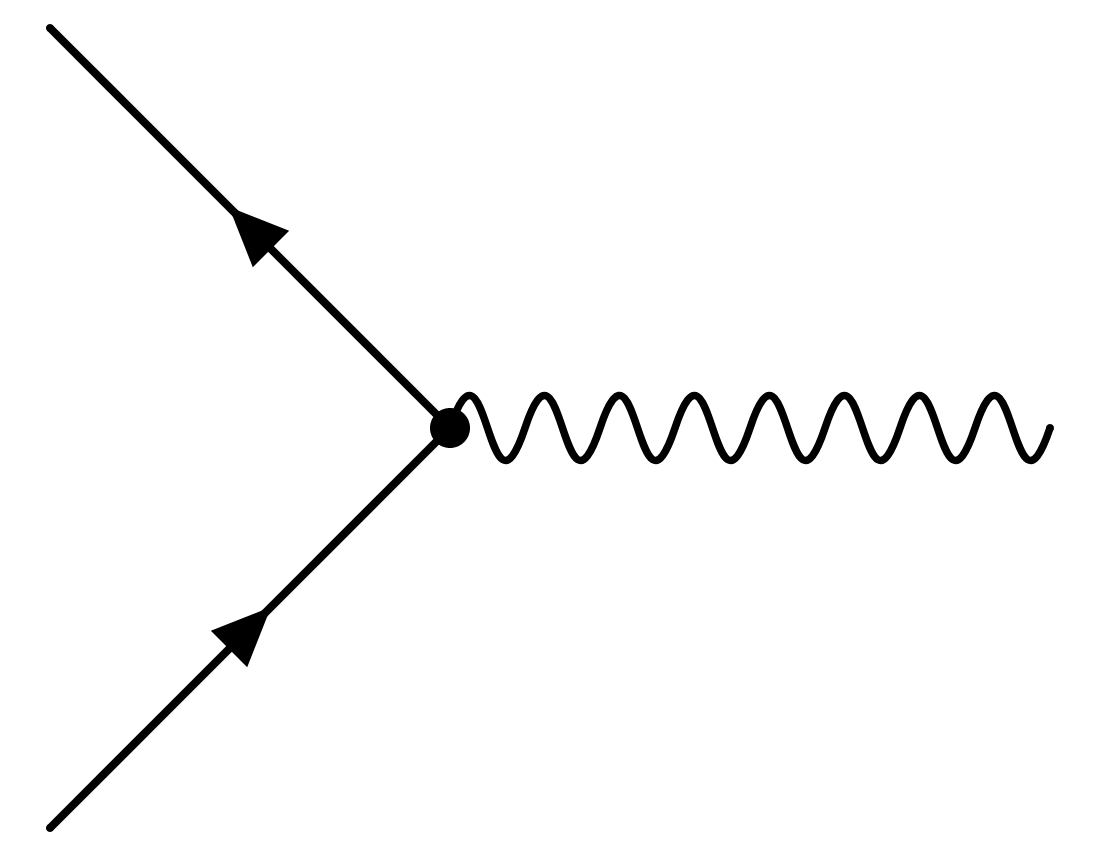
\includegraphics[width=0.27\textwidth]{qed_fundamental}
    \caption[]{The Fundamental interaction vertex of \ac{qed}. Two fermions interacting with a massless photon.}
    \label{fig:qed_fundamental}
\end{figure}
The dyanmics for the photon can be added with the spin-1 Proca Lagrangian from table \ref{tab:fields}. The $F_{\mu\nu}$ term is locally gauge invariant whereas $A_\mu A^\mu$ is not, since it picks up a second derivative for $\alpha$ and therefore is required to be massless. The full \ac{qed} lagrangian then reads
\begin{equation}
    \mathcal{L}_\mathrm{QED}
    =
    \underbrace{\overline{\psi}(i \gamma^\mu \partial_\mu - m )\psi}_{\mathcal{L}_\mathrm{Dirac} }
    +
    \underbrace{ e\overline{\psi} \gamma^\mu {\psi}A_\mu}_{\mathcal{L}_\mathrm{int}}
    -
    \underbrace{\frac{1}{4}F_{\mu\nu}F^{\mu\nu}}_{\mathcal{L}_\mathrm{Maxwell} }.
    \label{eq:l_qed}
\end{equation}
That this symmetry holds locally for all unitary $1\times1$ matrices $U(1)$ might seem extravagant, but the formalism is extendable to higher orders as for the \ac{ew} theory and \ac{qcd} case. The gauge group is abelian as any $1\times1$ matrix also commutes with itself.

\section{Quantum Chromodynamics}\label{sec:qcd}

Along the same lines as \ac{qed} is derived in section \ref{sec:qed}, the theory of the strong interactions \ac{qcd} is now a non-abelian gauge theory of the symmetry group $SU(3)$. The latter is generated by the $3\times 3$ Gell-Mann matrices $\lambda_a$ with $ a\in\{1,\mathellipsis,8\}$. The fundamental charge becomes color and each quark is a triplet of the three color fermion fields $\Psi_k=(\psi_r,\psi_g,\psi_b)^T$ for all quark flavors $k$. Local gauge invariance of the Lagrangian
\begin{equation}
    \mathcal{L} =
    \sum_k
    \begin{pmatrix}
        \overline{\psi}_r & \overline{\psi}_g & \overline{\psi}_b
    \end{pmatrix}
    (i \gamma^\mu \partial_\mu - m )
    \begin{pmatrix}
        \psi_r \\
        \psi_g \\
        \psi_b
    \end{pmatrix}
    =
    \sum_k
    \overline{\Psi}_k(i \gamma^\mu \partial_\mu - m )\Psi_k,
    \label{eq:dirac}
\end{equation}
means that the spinors are required to be invariant under the transformation
\begin{equation}
    \Psi_k(x) \rightarrow e^{i \alpha_a(x) \lambda_a/2} \Psi_k(x),\qquad \alpha\in\mathbb{R},\quad a\in\{1,\mathellipsis,8\},
\end{equation}
with $\alpha_a(x)$ a local phase and the index $a$ for the 8 gluons. It is noted here that summation over equal indices $\alpha_a(x) \lambda_a=\sum_i \alpha_a(x) \lambda_a$ is assumed. As in \ac{qed} a covariant derivative is introduced
\begin{equation}
    D_\mu = \partial_\mu - i g_s \frac{\lambda_a}{2}G_\mu^a,
\end{equation}
involving the eight gluon vector fields $G_\mu^a$ and the coupling strength $g_s$, which is related to the strong coupling constant as
\begin{equation}
    \alpha_s=\frac{g_s^2}{4\pi}.
\end{equation}
Again, self coupling terms are added
\begin{equation}
    G^a_{\mu\nu}=\partial_\mu G_\nu^a-\partial_\nu G_\mu^a+g_s f^a_{\beta\gamma}G^\beta_\mu G_\nu^\gamma, \qquad \text{with } [\lambda_a,\lambda_b]= i f_{ab}^c \lambda_c,
\end{equation}
to get the gauge invariant \ac{qcd} Lagrangian
\begin{align}
    {\mathcal {L}}_{\text{QCD}} & =\sum_k\overline{\Psi}_k\left( i \gamma^\mu D_\mu-m_k\right)\Psi_k-{\frac {1}{4}}G_{\mu \nu }^{a}G^{a\mu \nu}                                                                                    \\
                                & =\sum_k{\overline{\Psi}_k}\left(i\gamma^\mu \partial_\mu-m_k\right)\Psi_k+ g_s{\overline{\Psi}_k}\gamma ^{\mu }\frac{ \lambda_a}{2} \Psi_k G_\mu^a - {\frac {1}{4}}G_{\mu \nu }^{a}G^{a\mu \nu}.
    \label{eq:l_qcd}
\end{align}
This Lagrangian consists of a kinetic term for each quark, an interaction term of the quarks with the gluons and gluon-gluon interactions resulting in vertices shown in figure \ref{fig:qcd_vertices}. These interactions become apparent when $G^a_{\mu\nu}$ is squared, leading to cubic and quartic terms for the fields.
\begin{figure}[H]
    \centering
    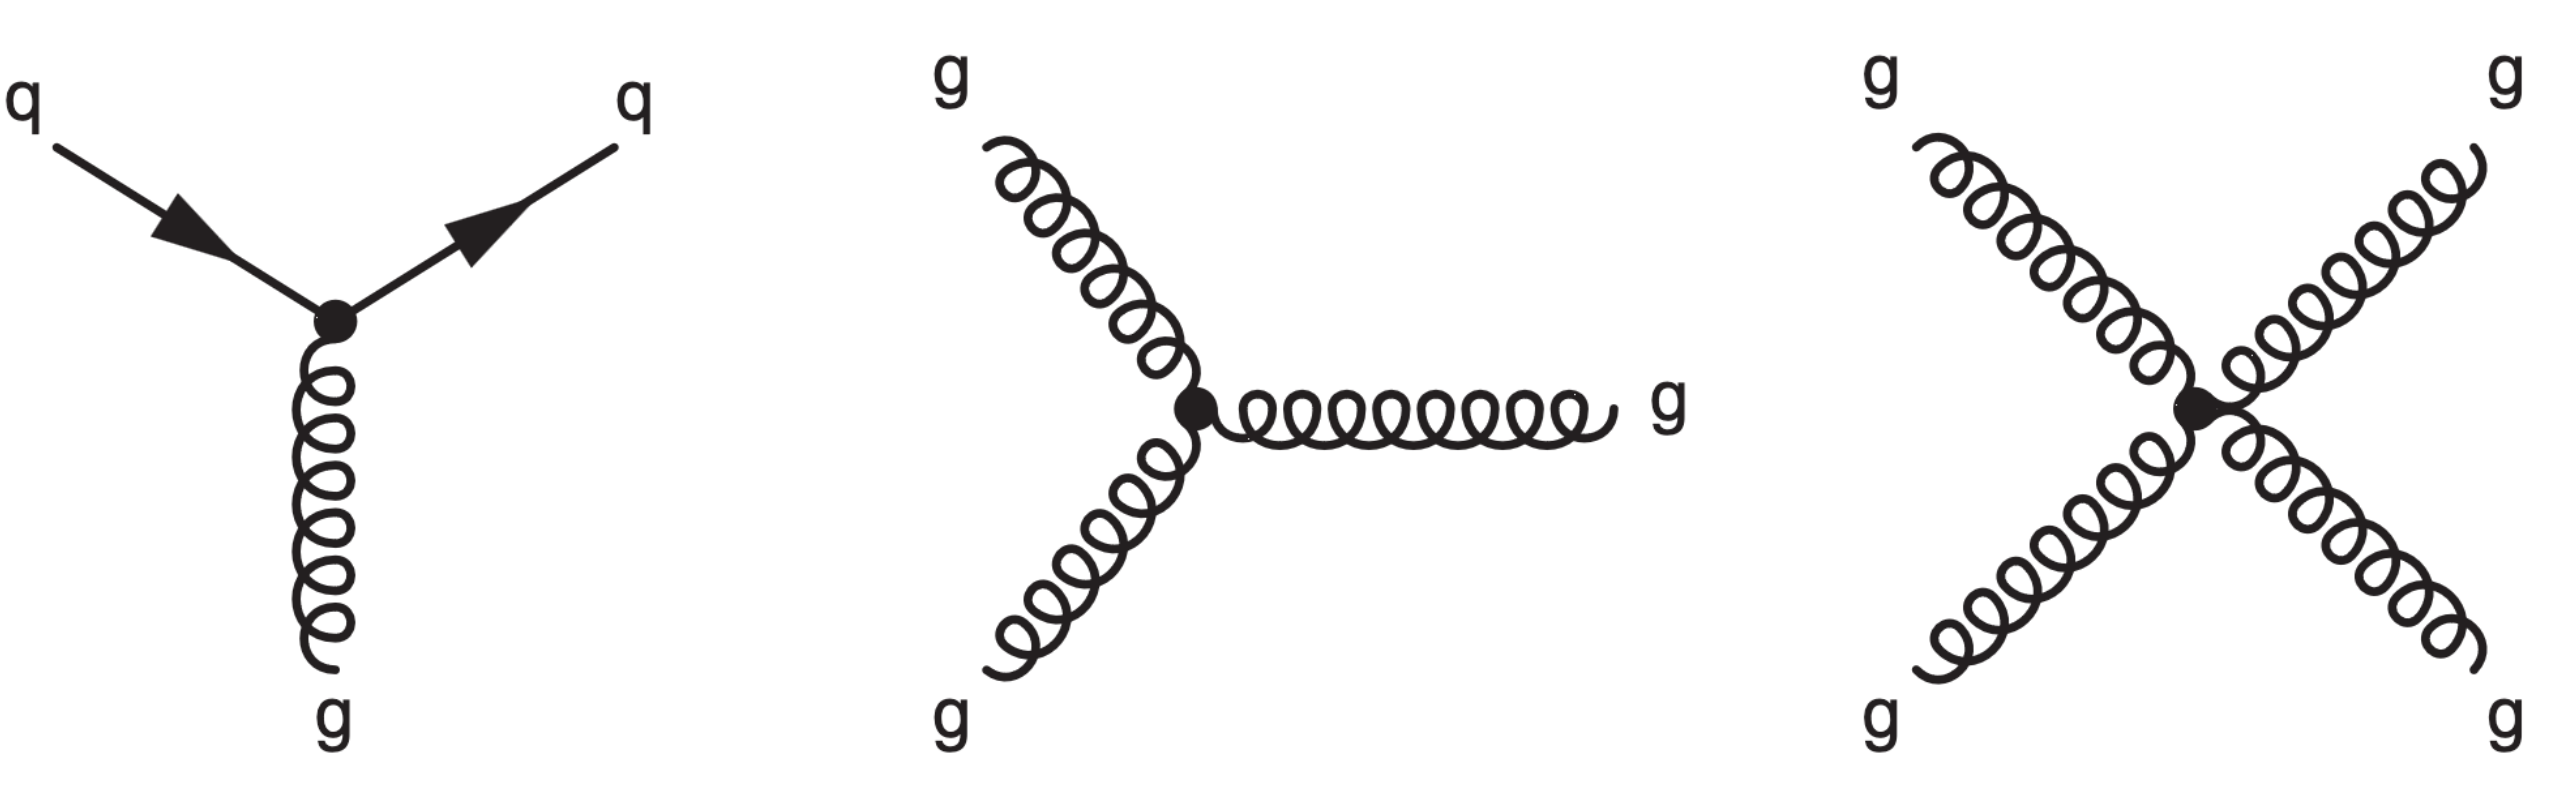
\includegraphics[width=0.8\textwidth]{gluon_gluon_interactions}
    \caption[]{(left) Quarks interacting with a gluon. (middle) triplet and (right) quartic self coupling of gluons. Adopted from \citep{thomson2013modern}.}
    \label{fig:qcd_vertices}
\end{figure}

\section{Renormalization}\label{sec:renormalization}
\begin{figure}
    \centering
    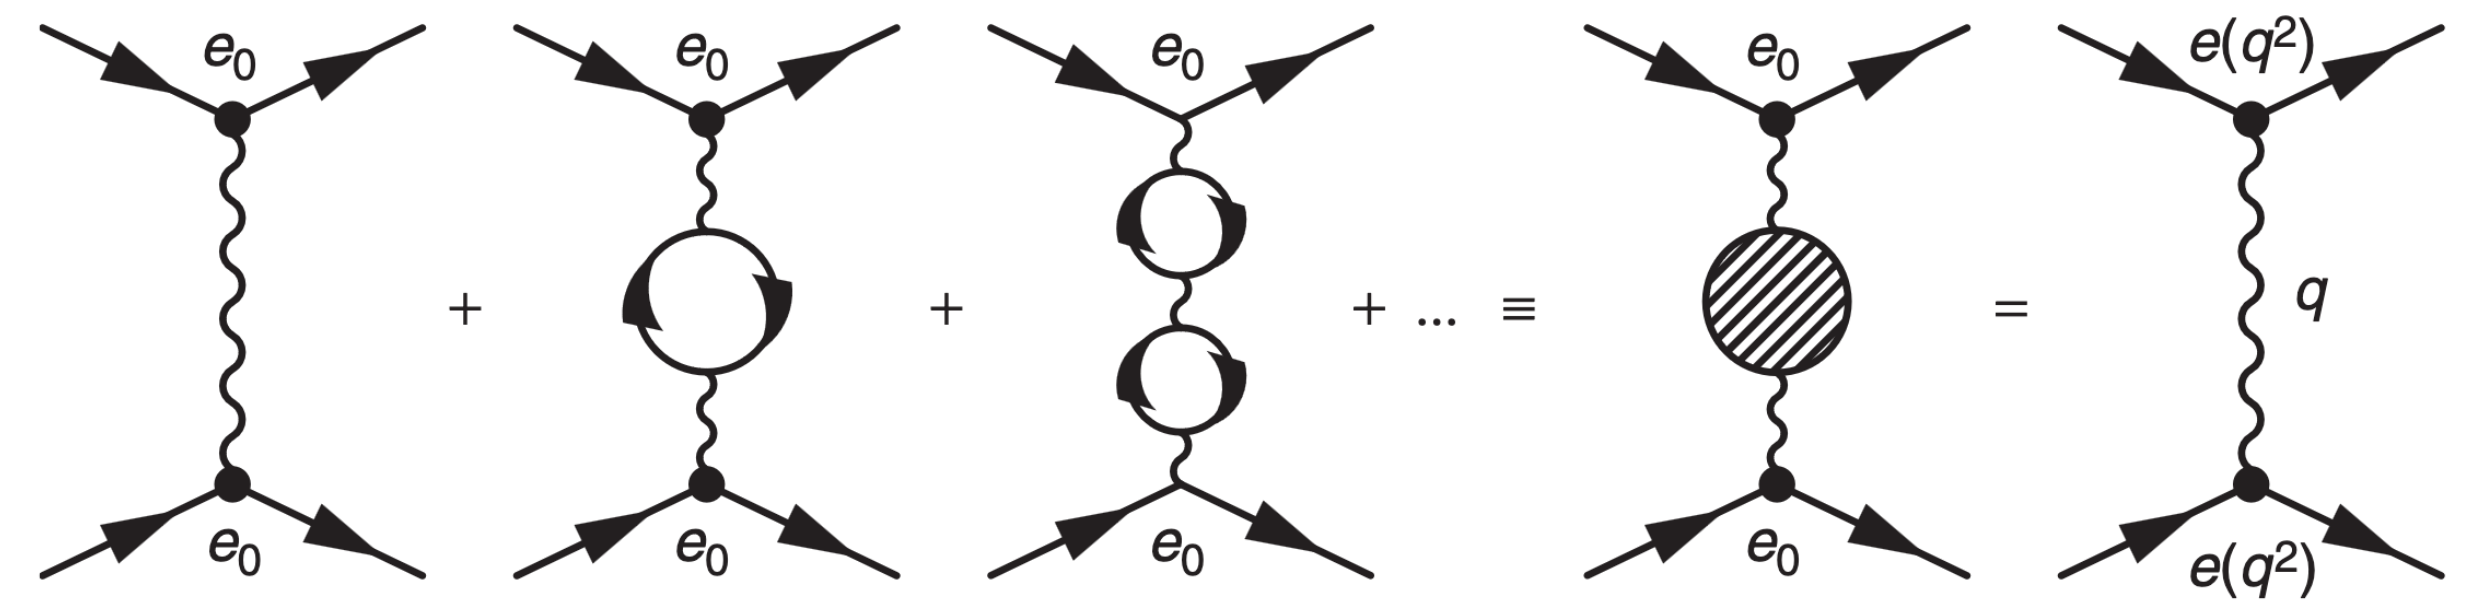
\includegraphics[width=1\textwidth]{qed_diagrams}
    \caption[]{Higher order loop corrections in \ac{qed} schematically treated as one effective diagram. Adopted from \citep{thomson2013modern}.}
    \label{fig:qed_diagrams}
\end{figure}
When attempting to calculate amplitudes $\mathcal{M}$ for higher-order diagrams in \ac{qed}, such as the second or third diagrams shown in Figure \ref{fig:qed_diagrams}, it results in diverging integrals. This phenomenon, known as vacuum polarization, occurs as virtual particle-antiparticle pairs act to screen the actual charge of the electron $e0$, analogous to a dielectric medium in classical electrodynamics. To address this issue, an effective charge/coupling $e(q^2)$ is introduced. This coupling becomes a function of the squared four-momentum $q^2$ at the virtual photon vertex, as depicted in Figure \ref{fig:qed_diagrams} and renders the integrals finite.

For the second diagram in figure \ref{fig:qed_diagrams} with only one loop correction, it can be shown that for some measured coupling $e(q^2=\mu^2)$ at an energy scale $\mu^2$, the actual coupling $e(q^2)$ follows a scaling behavior that holds if $q^2$ and $\mu^2$ are larger than the electron mass \citep{thomson2013modern}. The coupling constant is now a running coupling $e(q^2)$ and reads in terms of the fine structure constant $\alpha(q^2)=e^2(q^2)/4\pi$,
\begin{equation}
    \alpha(q^2)=
    \frac{\alpha(\mu^2)}
    {1-\alpha(\mu)\frac{1}{3\pi}
        \ln
        \left(\frac{q^2}{\mu^2}\right)}.
    \label{eq:qed_coupling}
\end{equation}
Therefore with increasing momentum transfer, or a closer approach in a collision, the number of virtual pair production processes is effectively reduced, revealing the bare charge of the electron. This behavior is shown qualitatively in figure \ref{fig:renorm_scaling}(a).
\begin{figure}
    \centering
    \subfigure[]{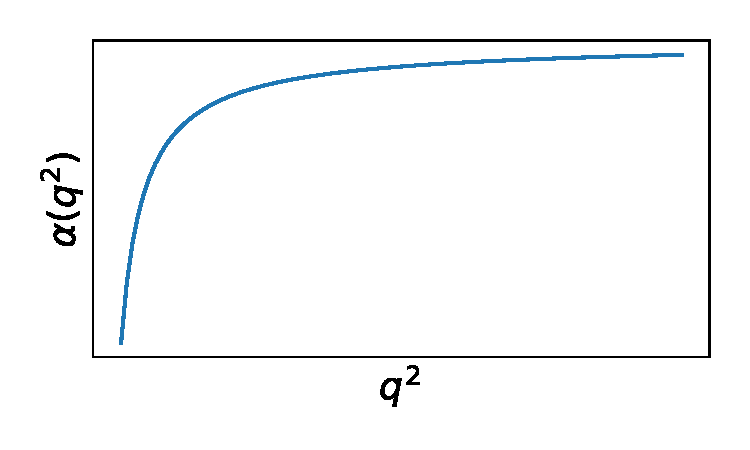
\includegraphics[width=.49\textwidth]{qed_scaling}}
    \subfigure[]{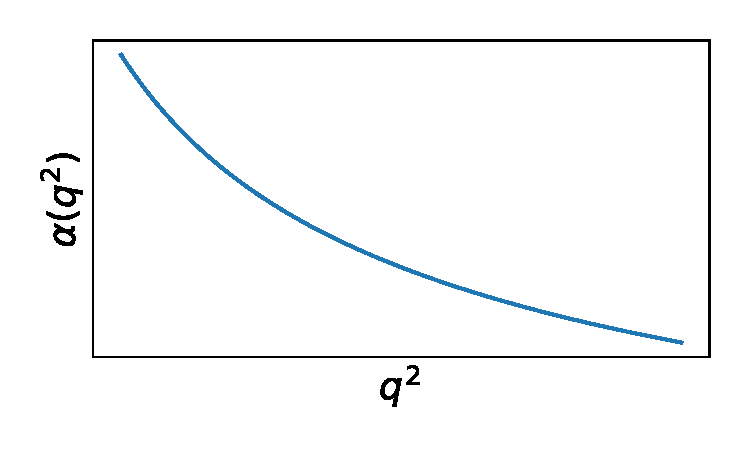
\includegraphics[width=.49\textwidth]{qcd_scaling}}
    \caption[]{Qualitative behavior of the running couplings for (\textbf{a}) \ac{qed} as of equation \ref{eq:qed_coupling} and (\textbf{b}) \ac{qcd} as of equation \ref{eq:qcd_coupling}.}
    \label{fig:renorm_scaling}
\end{figure}
\begin{figure}[H]
    \centering
    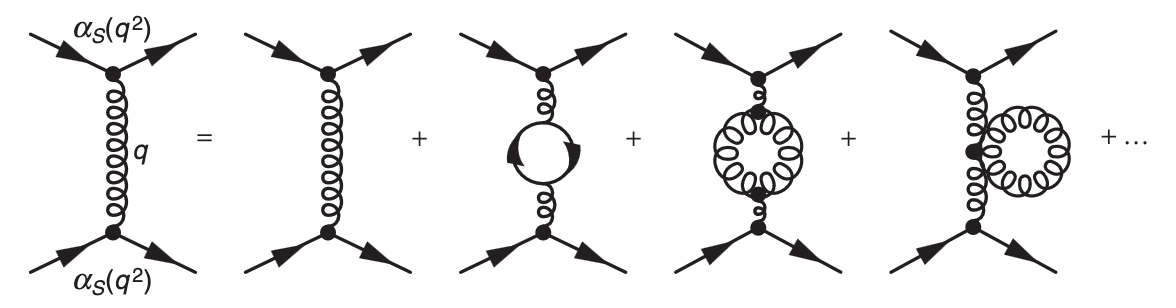
\includegraphics[width=1\textwidth]{qcd_diagrams}
    \caption[]{Some higher order loop corrections in \ac{qcd}. Adopted from \citep{thomson2013modern}.}
    \label{fig:qcd_diagrams}
\end{figure}
Renormalization in \ac{qcd} can be derived similarly but also the quartic and triplet couplings exemplified in figure \ref{fig:qcd_diagrams} need to be considered that result in a scaling for the strong coupling
\begin{equation}
    \alpha_S(q^2)=
    \frac{\alpha_S(\mu^2)}
    {1+B\alpha_S(\mu)
        \ln
        \left(\frac{q^2}{\mu^2}\right)}, \qquad \text{with } B=\frac{11N_c-2N_f}{12\pi}.
    \label{eq:qcd_coupling}
\end{equation}
For 3 color charges $N_c$ and 6 fermions $N_f$ in the \ac{sm}, $B$ is positive and the coupling becomes weaker for shorter scales or higher momentum transfer as can be seen in figure \ref{fig:renorm_scaling}(b).

The fine structure constant of \ac{qed} $\alpha(q^2\approx 0)\approx 1/137$ does not vary dramatically over the energy ranges of matter for particle physics as shown in figure \ref{fig:renorm_scaling_exp}(a).
\begin{figure}
    \centering
    \subfigure[]{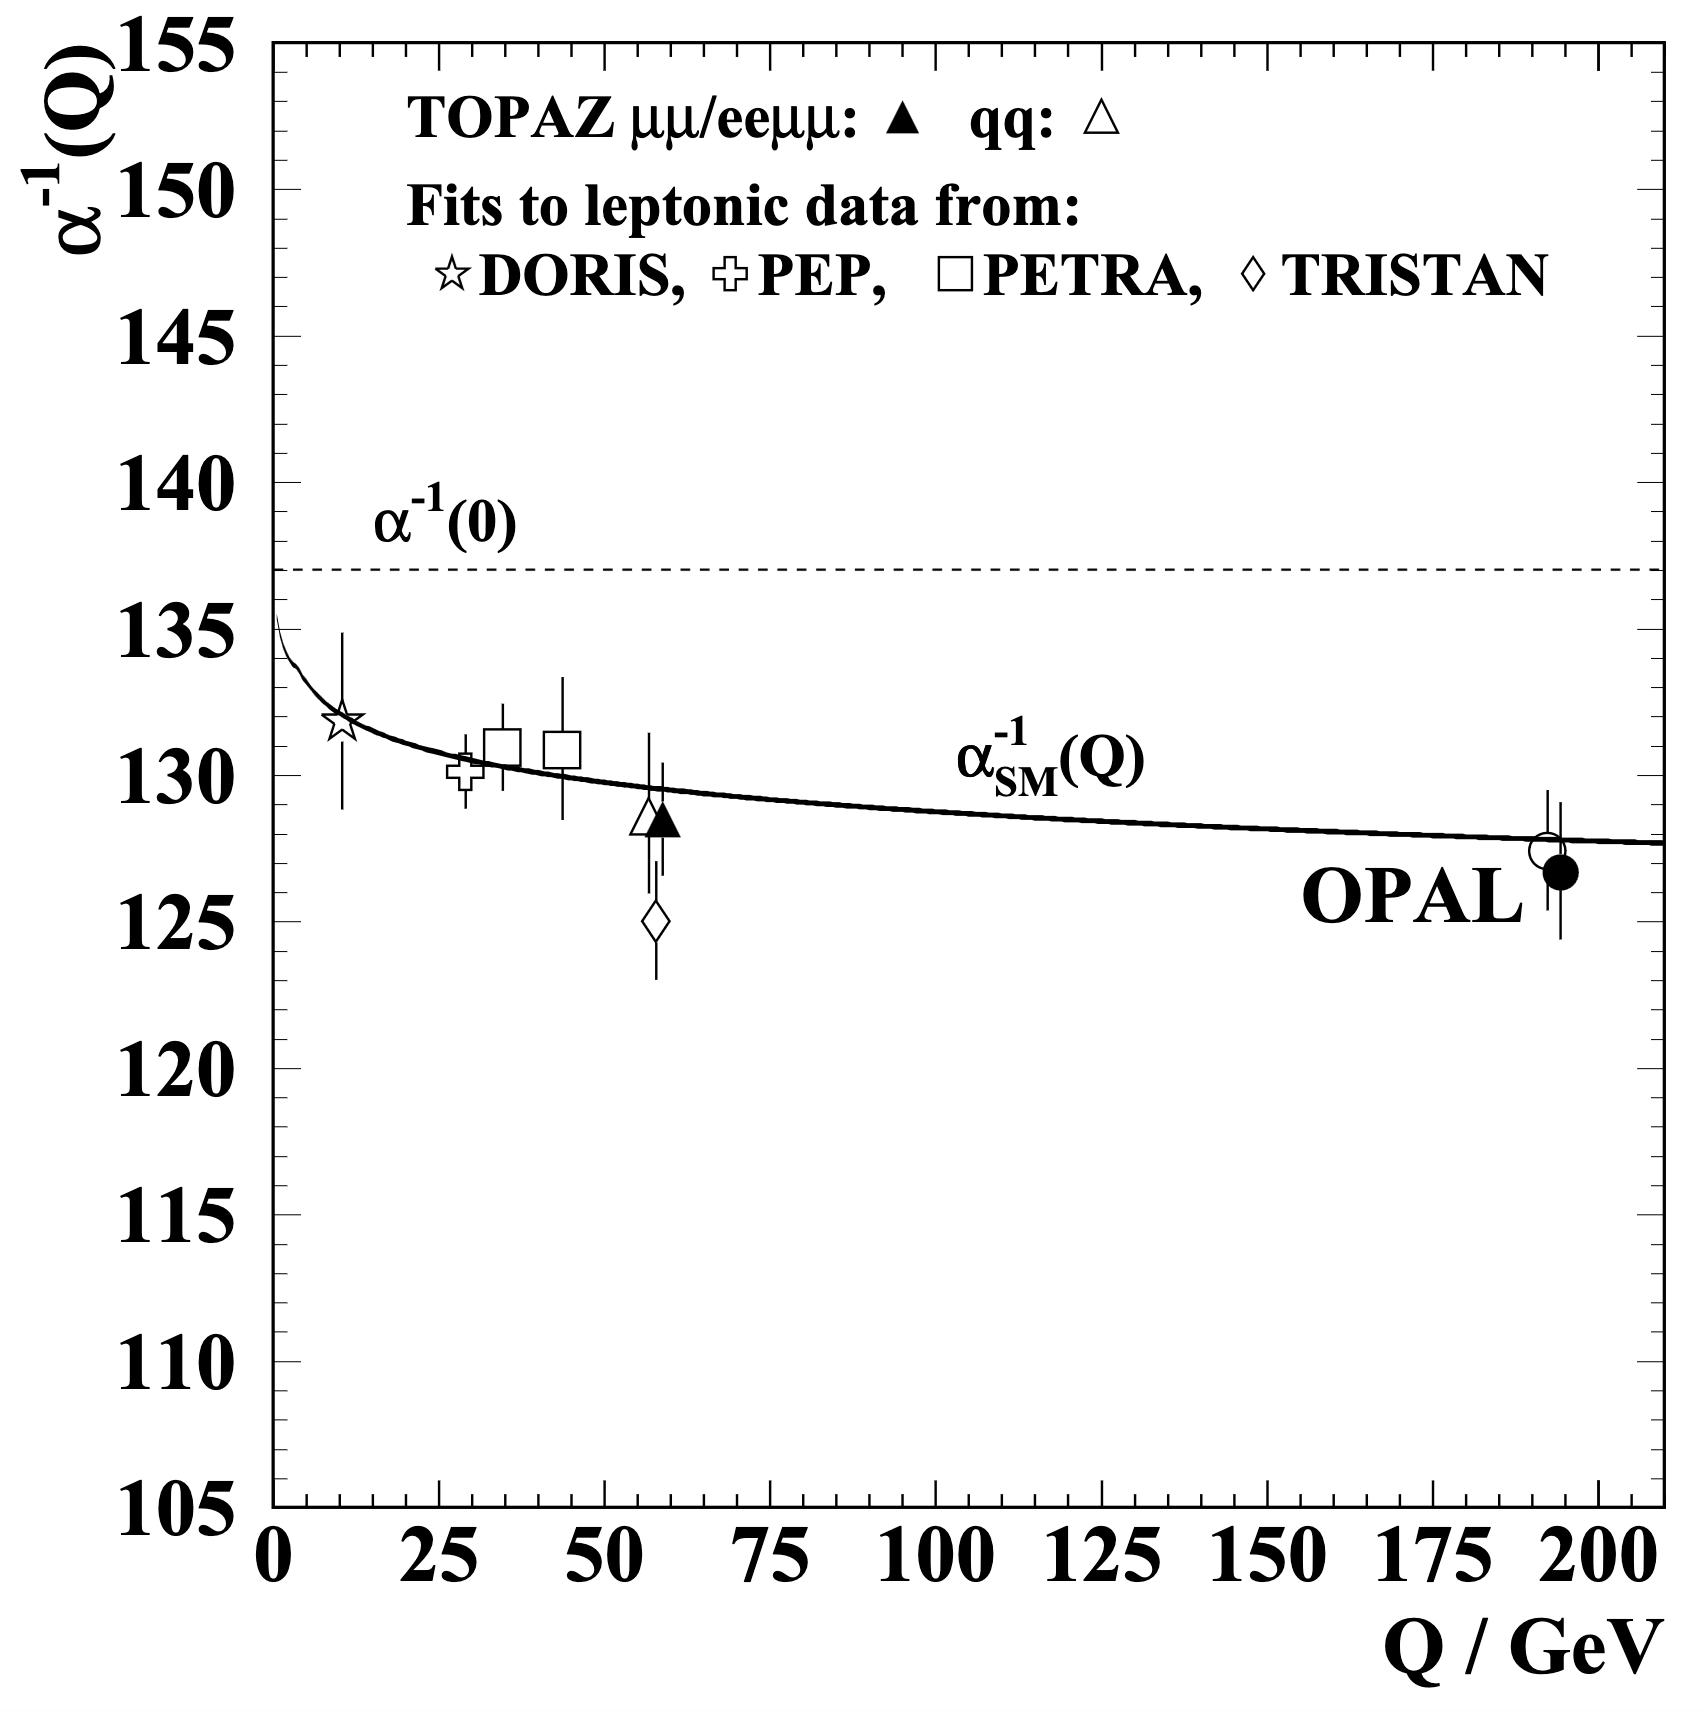
\includegraphics[width=.47\textwidth]{qed_scaling_experiment}}\hspace{5mm}
    \subfigure[]{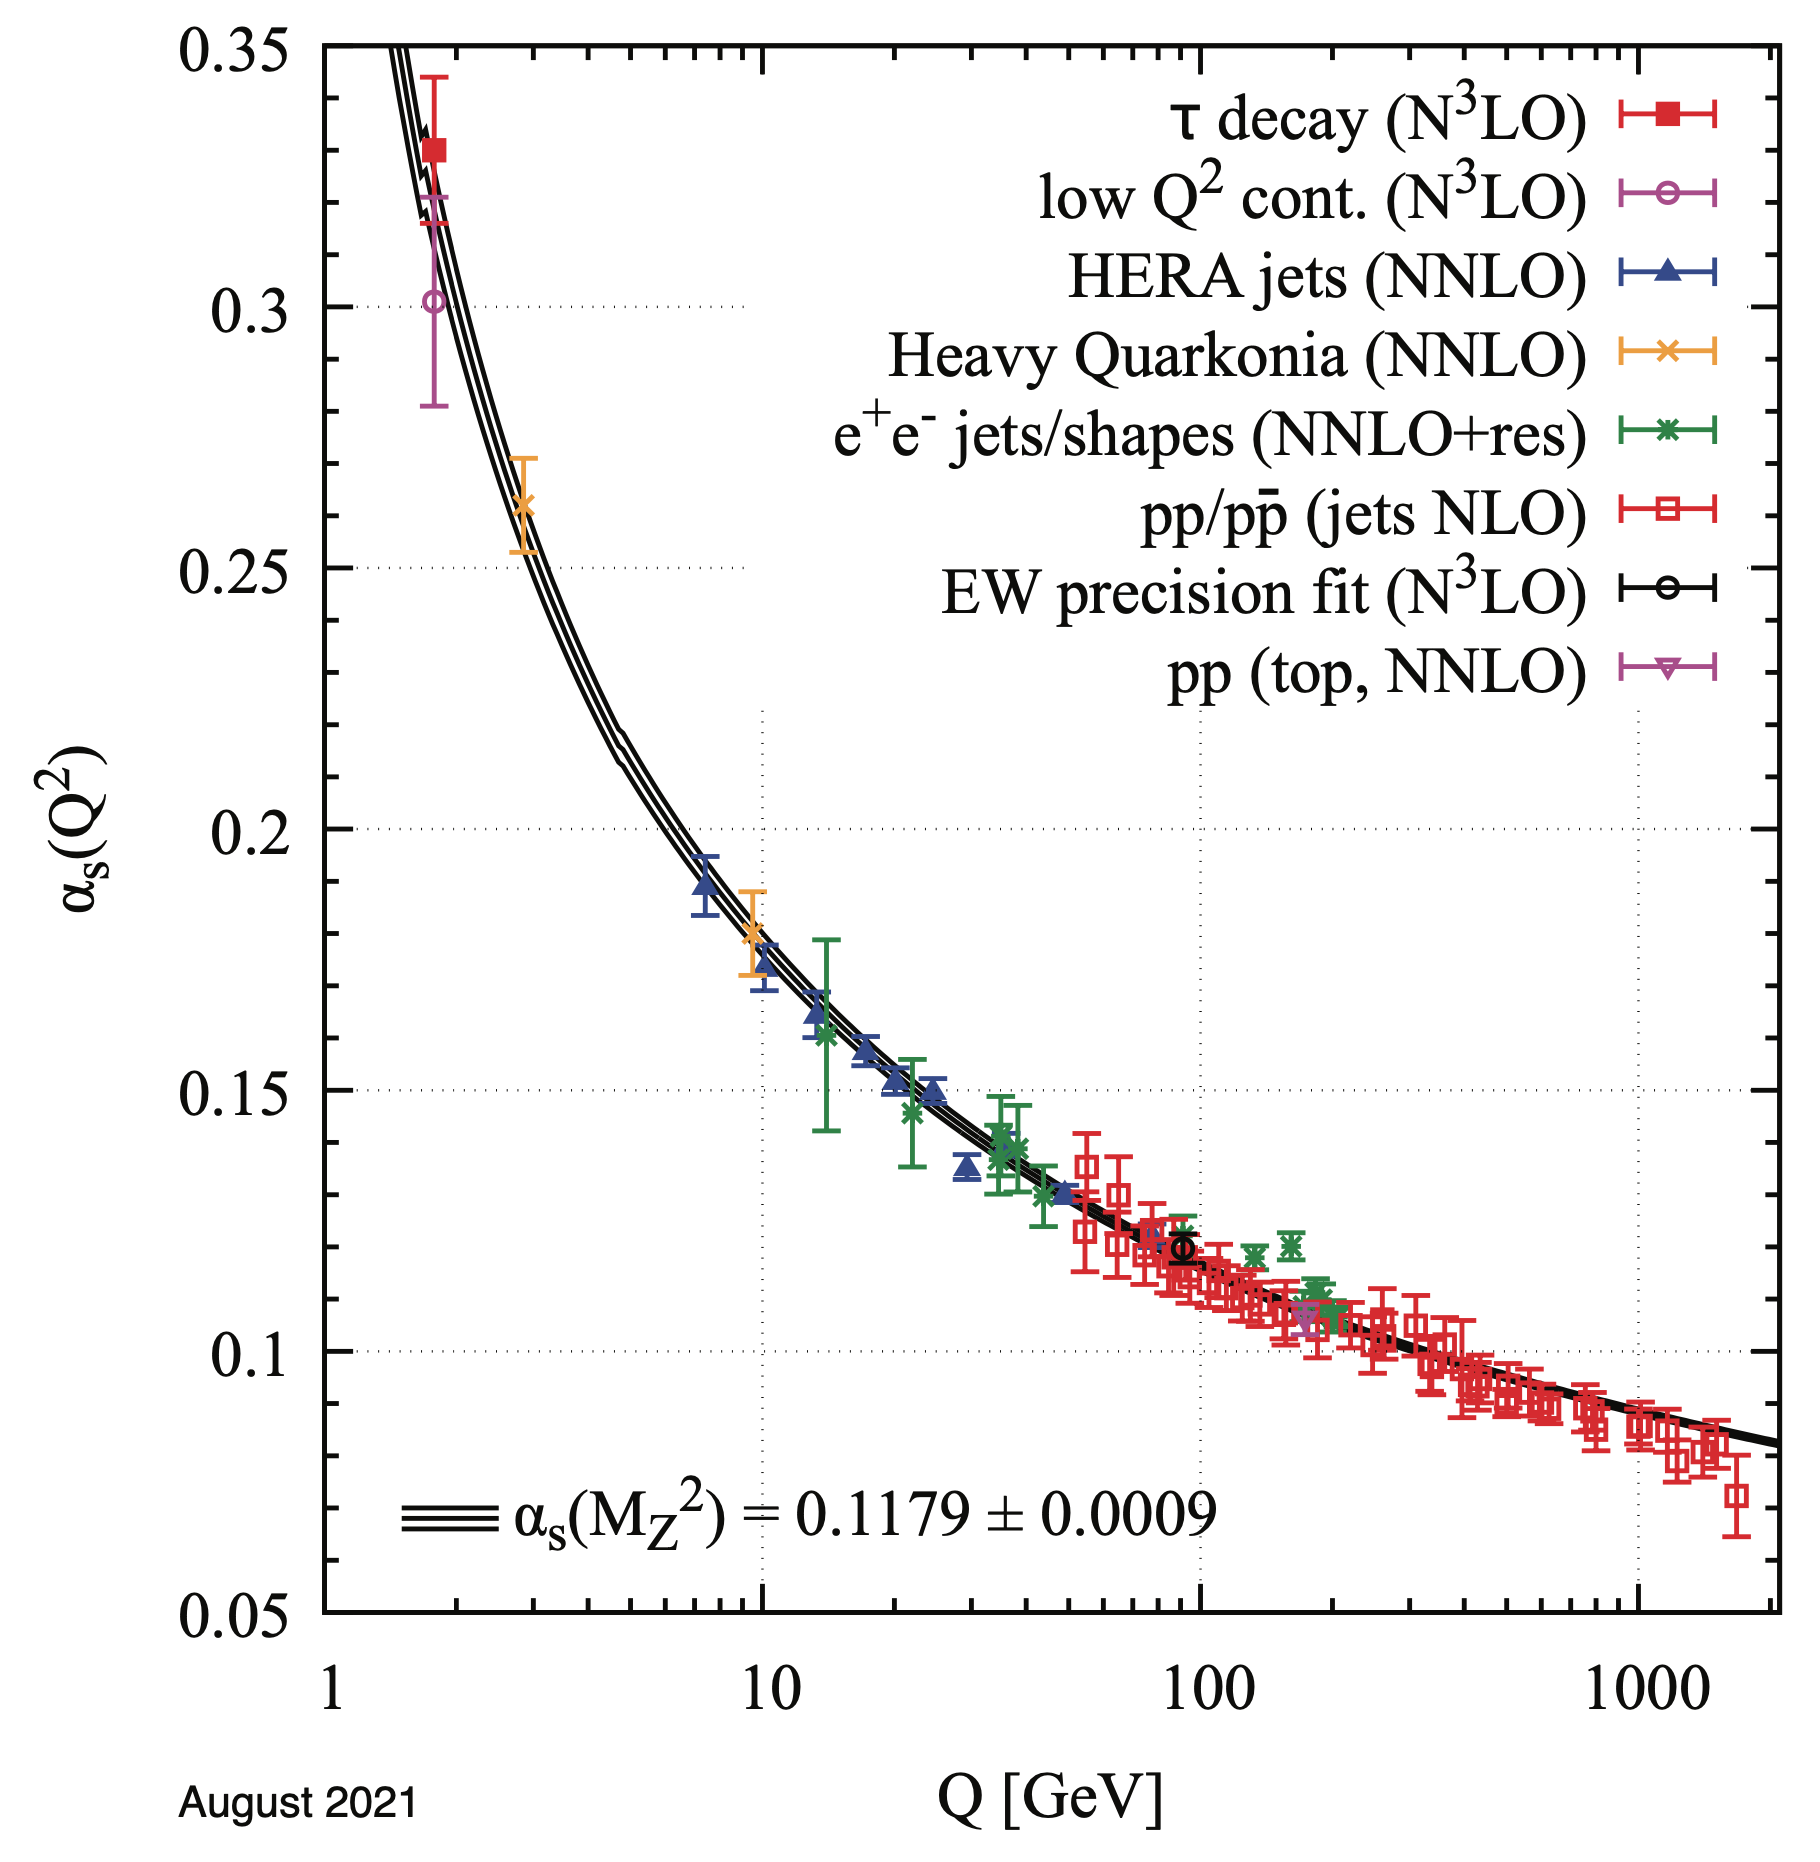
\includegraphics[width=.47\textwidth]{qcd_scaling_experiment}}
    \caption[]{Measurements of the running couplings for (\textbf{a}) \ac{qed} (note the inverted coupling on the y-axis) adopted from \citep{opal2004tests} and (\textbf{b}) \ac{qcd} adopted from \citep{particle2022review}.}
    \label{fig:renorm_scaling_exp}
\end{figure}
Most importantly the running coupling of \ac{qed} does not impact the perturbative approach outlined in section \ref{sec:qft} since $\alpha\ll1$. This is not the case for \ac{qcd} where $\alpha_S$ at $q\approx\qty{1}{GeV}$ is of $\mathcal{O}(1)$ and perturbation theory breaks down for calculations on bound hadronic states and latter processes in hadronization es explained below. While perturbation theory for \ac{qcd} remains valid for $\alpha_S\gtrsim  0.1$, which corresponds to $q\gtrsim \qty{100}{GeV}$, for basically all \ac{qcd} calculations at the \ac{lhc}, higher order corrections must be considered.

The behavior of the running coupling in \ac{qcd} is called asymptotic freedom, since the theory is free of asymptotics/divergences with increasing energy scale or decreasing distance. In turn to the photon in \ac{qed}, gluons carry charge and thus attempting to separate quarks results in additional gluons contributions to the interaction, increasing both the energy and force between the quarks. Eventually, it becomes energetically favorable to create a quark-antiquark pair from the vacuum, which then bind with the separating quarks to form new, color-neutral hadrons. This is also known as color confinement, which states that colored particles can only be observed in bound states.


\section{Electroweak Unification}\label{sec:ew}
The weak force can be incorporated into a gauge-invariant formalism by using a $SU(2)$ symmetry. This is further combined with the electromagnetic force to derive a unified framework for both forces, known as the electroweak interaction, which is described by the symmetry group $SU(2)_L \otimes U(1)_Y$. In this framework, the weak force interacts exclusively with left-handed chiral states of particles, such as for a left-handed fermion $\psi_L$ as expanded on below. Fermions can be grouped by their characteristics into left handed doublets
\begin{equation}
    \begin{pmatrix}
        \nu_e \\ e
    \end{pmatrix}_L, \;
    \begin{pmatrix}
        \nu_\mu \\ \mu
    \end{pmatrix}_L, \;
    \begin{pmatrix}
        \nu_\tau \\ \tau
    \end{pmatrix}_L, \;
    \begin{pmatrix}
        u \\ d
    \end{pmatrix}_L, \;
    \begin{pmatrix}
        c \\ s
    \end{pmatrix}_L, \;
    \begin{pmatrix}
        t \\ b
    \end{pmatrix}_L, \;
    \label{eq:weak_doublets}
\end{equation}
with weak isospin $I=1/2$ that has as third component $I_3=\pm1/2$ for the upper and lower doublet particle respectively. In contrast the weak hypercharge $Y$ is associated to right handed singlets
\begin{equation}
    e_R    ,\quad \mu_R ,\quad    \tau_R ,\quad    u_R,\quad d_R ,\quad    c_R ,\quad s_R ,\quad    t_R ,\quad b_R,
\end{equation}
with $I=0$. The relation between the electric charge of the particle and these quantum numbers is governed by the Gell-Mann-Nishijima Formula
\begin{equation}
    Q=I_3+Y/2.
    \label{eq:gellmann_nishijima_formula}
\end{equation}
The electroweak Lagrangian is then composed of four basic terms
\begin{equation}
    \mathcal{L}_\mathrm{EW} = \mathcal{L}_\mathrm{fermions}+\mathcal{L}_\mathrm{gauge}+\mathcal{L}_\mathrm{Higgs}+\mathcal{L}_\mathrm{Yukawa}.
    \label{eq:L_EW}
\end{equation}
Following the same steps as for \ac{qcd} and \ac{qed} the Lagrangian can be rendered gauge invariant by introducing a covariant derivative and gauge fields that are dictated by the group symmetry.

$SU(2)$ is generated through the three Pauli matrices $\bm{\sigma}$ requiring 3 vector gauge fields $W^a_\mu$, $a=\{1,2,3\}$ whereas the $U(1)$ symmetry of the vector gauge field $B_\mu$ is generated by the weak hypercharge $Y$ so the Lagrangian needs to be invariant under the transformation
\begin{align}
    \psi_{L} & \rightarrow e^{i \alpha_a(x) \sigma_a/2}e^{ iY/2} \psi_{L},\qquad & a\in\{1,\mathellipsis,3\} ,\quad \alpha\in\mathbb{R} & \label{eq:gauge_transformation_left}
    \\
    \psi_{R} & \rightarrow e^{ i\beta(x) Y/2} \psi_{R},\qquad                    & \beta\in\mathbb{R}                                   & \label{eq:gauge_transformation_right}
\end{align}
% At this stage the new vector fields are still massless and give the fermionic and gauge parts of the Lagrangian and will be explained below. The masses for the fermions and bosons can be incorporated via the Higgs mechanism that is described in section \ref{sec:higgs_mechanism} yielding the Higgs and Yukawa parts of the Lagrangian.


\subsubsection*{Fermion term}
To distinguish left- and right handed particle states the according spinors can be written as
\begin{equation}
    \psi_L=\frac{1-\gamma^5}{2}\psi, \quad \psi_R=\frac{1+\gamma^5}{2}\psi.
\end{equation}
The concept of helicity, which is the projection of a particle's spin along its momentum direction, helps in understanding these states. $\psi_{L,R}$ however are not helicity eigenstates but rather select the spinor $\psi$ with corresponding helicity and vanish otherwise
\begin{equation}
    \frac{1}{2}(1 \pm y^5)\psi =
    \begin{cases}
        0    & \text{if } \psi \text{ has helicity } \mp1, \\
        \psi & \text{if } \psi \text{ has helicity } \pm1.
    \end{cases}\label{eq:left_handed_state}
\end{equation}
The aforementioned doublets and singlets are then represented by
\begin{equation}
    \psi_L^j=
    \begin{pmatrix}
        \psi_{L+}^j \\ \psi_{L-}^j
    \end{pmatrix},
    \quad \psi_{R\xi}^j,
\end{equation}
with $j$ running over the doublets from equation \ref{eq:weak_doublets} and $\xi=+$ for u-type fermions and $\xi=-$ for d-type fermions.
The covariant derivative is
\begin{align}
    D_\mu^L & =\partial_\mu- i g_2 \frac{{\sigma}_a}{2}W_\mu^a+i g_1\frac{Y}{2}B_\mu, \label{eq:cov_diff_L} \\
    D_\mu^R & =\partial_\mu+ i g_1\frac{Y}{2}B_\mu,
\end{align}
with coupling $g_2$ and $g_1$ to the vector fields and $\sigma_a$ for the corresponding Pauli matrix, so that the fermionic part of the Lagrangian becomes
\begin{equation}
    \mathcal {L}_\text{fermions} = \sum_j\overline{\psi}^j_L i \gamma^\mu D_\mu^L\psi_L^j+\sum_{j,\xi}\overline{\psi}^j_{R\xi} i \gamma^\mu D_\mu^R\psi_{R\xi}^j.
    \label{eq:L_fermion}
\end{equation}

\subsubsection*{Gauge term}
The gauge field self interaction terms are
\begin{align}
    W_{\mu\nu}^a & =\partial_\mu W_\nu^a-\partial_\nu W_\mu^a+g_2\epsilon_{abc}W_\mu^b W_\nu^c, \\
    B_{\mu\nu}   & =\partial_\mu B_\nu-\partial_\nu B_\mu,
\end{align}
with $g_2$ the weak coupling constant and $\epsilon_{abc}$ the totally asymmetric Levi-Civita tensor yielding the gauge field part of the Lagrangian
\begin{equation}
    \mathcal {L}_\text{gauge} = -\frac{1}{4} W_{\mu\nu}^a W^{\mu\nu,a} - \frac{1}{4}B_{\mu\nu}B^{\mu\nu}.
\end{equation}
So far the \ac{ew} Lagrangian made of the fermions and gauge part describes massless fermions and gauge fields $W^a_\mu$. Up to this point, naive mass terms for the fields listed in Table \ref{tab:fields} have been deliberately omitted as they would break gauge invariance. The introduction of masses will be addressed through the Higgs mechanism and Yukawa couplings in the subsequent sections.

% A Proca mass term $\frac{1}{2} m^2 B_\mu B^\mu$ is not invariant as discussed in section \ref{sec:qed}. For a Dirac term like $-m\overline{\psi}\psi$ this can be seen by rewriting it in terms of the left-handed and right-handed fields by inserting a 1 for e.g. the electron and exploiting the transformation of chiral states as of equation \ref{eq:left_handed_state}
% \begin{equation}
%     -m\overline{e}e =
%     -m\overline{e} \left[\frac{1}{2}(1-y^5)+\frac{1}{2}(1+y^5)\right]e
%     =-m(\overline{e}_R e_L+\overline{e}_L e_R).
%     \label{eq:yukawa_mass_term}
% \end{equation}
% $\overline{e}_R$ is a $SU(2)$ singlet and $e_L$ is one component of a $SU(2)$ doublet and therefore such a term is not gauge invariant. 


\section{Higgs Mechanism}\label{sec:higgs_mechanism}

In the previous sections, it was shown that the principle of local gauge invariance applied to the free Dirac Lagrangian can generate all the dynamics for a given interaction. However, this assumes that the accompanying gauge boson vector fields are massless, which is not the case for the weak interactions. The Higgs mechanism adds a field to the Lagrangian that provides mass terms for the vector bosons and fermions while preserving the principle of local gauge invariance. A way to implement this for a $U(1)$ symmetry is to consider two scalar fields $\phi_1$ and $\phi_2$ and combine them into a complex scalar field
\begin{equation}
    \phi (x)=\frac{1}{\sqrt{2}}(\phi_1(x)+i\phi_2(x)).
\end{equation}
A Lagrangian with a kinetic term $T(\phi)$ and a potential $V(\phi)$ with parameters $\mu$ and $\lambda$ can then be written as
\begin{equation}
    \mathcal{L}=T(\phi)-V(\phi)=
    \left[\left(\partial_\mu\phi\right)^* (\partial^\mu\phi)\right]
    -\left[
        -\mu^2(\phi^*\phi)+\lambda(\phi^*\phi)^2
        \right].
\end{equation}
This Lagrangian can be made locally gauge invariant under a $U(1)$ symmetry by following the transformation steps used in \ac{qed} from section \ref{sec:qed} by replacing the derivative with the covariant derivative with some vector field $B_\mu$ and coupling $g$
\begin{equation}
    \partial_\mu \rightarrow D_\mu = \partial_\mu + ig B_\mu.
\end{equation}
The transformations for the scalar and gauge fields are given as
\begin{align}
    \phi(x)  & \rightarrow  e^{i g\alpha(x)}\phi(x), \label{eq:scalar_local_gauge} \\
    B_\mu(x) & \xrightarrow{} B_\mu(x) -\partial_\mu\alpha(x).
\end{align}
The lowest energy state of a \ac{qft} is the vacuum state and therefore its eigenvalue is also called \ac{vev}. Here it is the one that minimizes the potential $V(\phi)$
\begin{equation}
    v =
    \begin{cases}
        0                                                     & \lambda>0, \mu^2<0  \\
        \sqrt{\phi_1^2+\phi_2^2}=\sqrt{\frac{\mu^2}{\lambda}} & \lambda>0, \mu^2>0,
    \end{cases}
\end{equation}
and is either 0 or forms an infinite set of minima as illustrated in figure \ref{fig:higgs_potential} by the dashed circle.
\begin{figure}
    \centering
    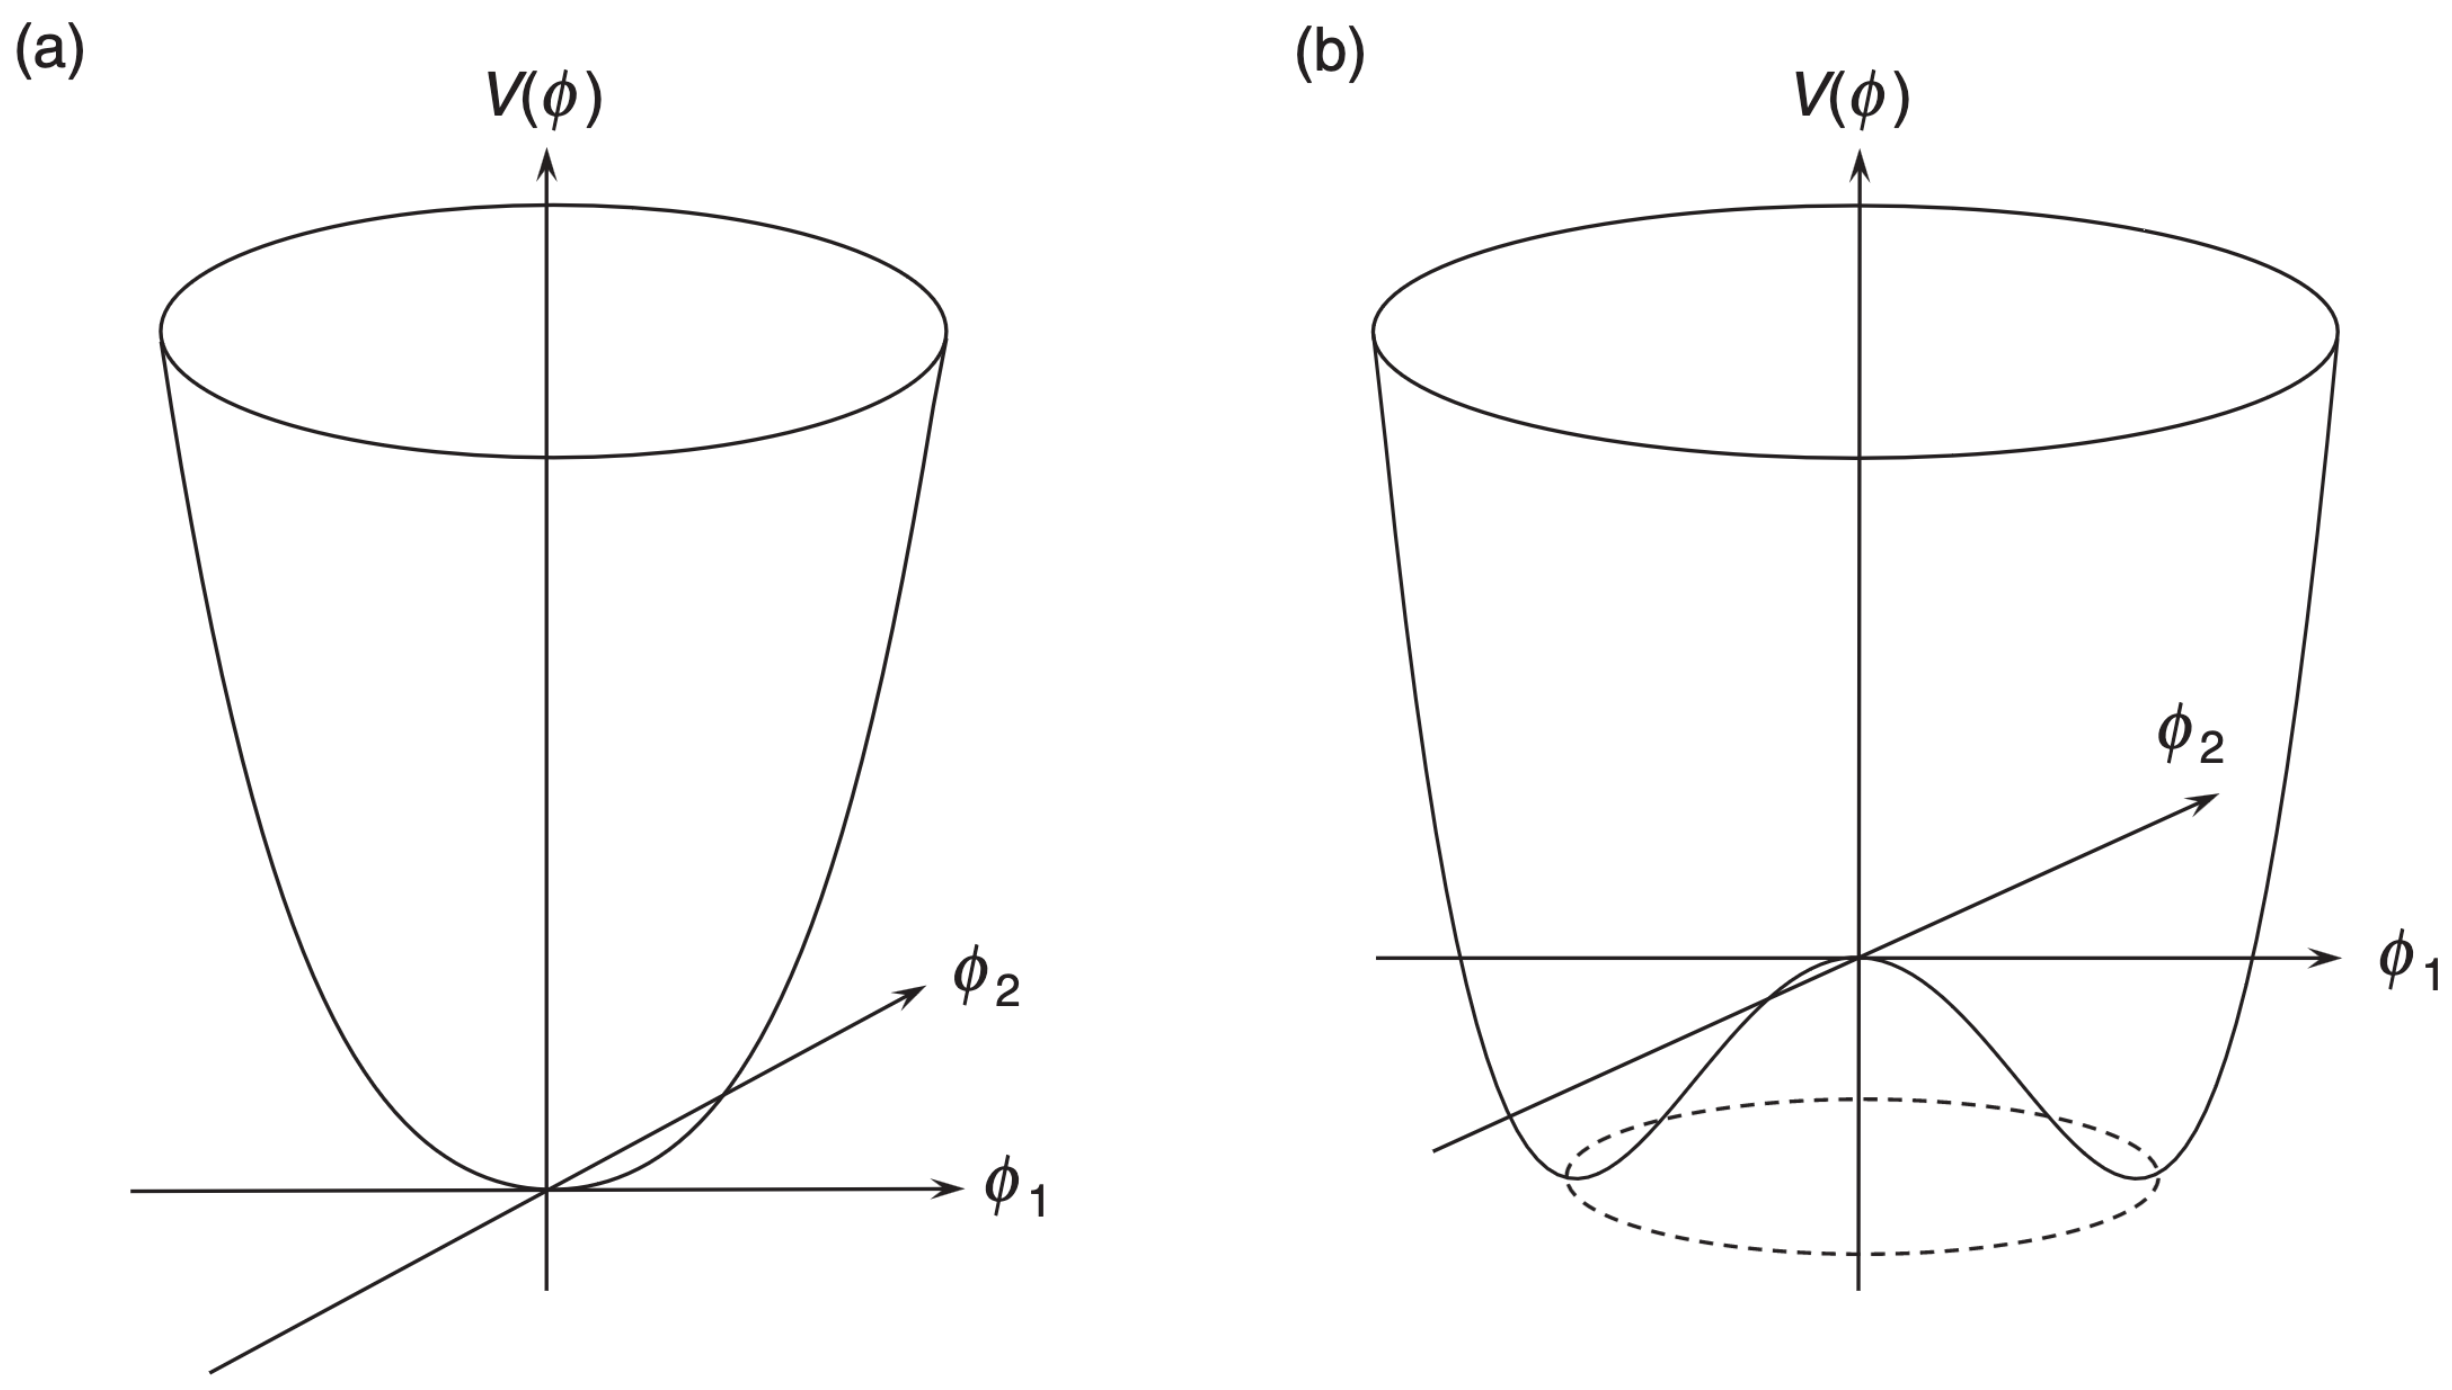
\includegraphics[width=.8\textwidth]{higgs_potential}
    \caption[]{Potential $V(\phi)$: (\textbf{a}) for $\lambda>0$ and $\mu^2<0$ and (\textbf{b}) for values $\lambda>0$ and $\mu^2>0$. Adopted from \citep{thomson2013modern}.}
    \label{fig:higgs_potential}
\end{figure}

The \ac{qft} perturbation ansatz from section \ref{sec:qft} starts from perturbations around the ground state. Thus for the ansatz to work with the $\mu^2>0$ case new field variables $\eta(x)$ and $\xi(x)$ can be introduced so the perturbation calculus can be applied about the ground state
\begin{equation}
    \phi_1(x)=v+\eta(x),\quad \phi_2(x)=\xi(x).
\end{equation}
The physical vacuum state spontaneously breaks the symmetry of the Lagrangian. Furthermore the physical predictions of the Lagrangian do not depend on the choice of the gauge and can be chosen in a way that it eliminates the field $\xi (x)$. In particular, if $\alpha(x)=-\xi(x)/(gv)$, the transformation from equation \ref{eq:scalar_local_gauge} can be made unitary ($UU^\dagger=1$) when expressed to first order in the field variables. Moreover $\eta(x)$ can then be reinterpreted as the Higgs field $h(x)$
\begin{equation}
    \phi(x)  \rightarrow  e^{i g\alpha(x)}\frac{1}{\sqrt{2}}(v+\eta(x)+i\xi(x))
    \approx
    \frac{1}{\sqrt{2}}e^{-i \frac{\xi(x)}{v}}[v+\eta(x)]e^{i\frac{\xi(x)}{v}}
    =
    \frac{1}{\sqrt{2}}(v+h(x)).
\end{equation}
The full locally gauge invariant Lagrangian for a $U(1)$ complex scalar field then reads except for constants
\begin{align}
    \mathcal{L}= &
    \underbrace{\frac{1}{2}(\partial_\mu h)(\partial^\mu h)-\lambda v^2 h^2}_{\text{massive h scalar}}
    -
    \underbrace{\frac{1}{4}F_{\mu\nu}F^{\mu\nu} -\frac{1}{2}g^2v^2 B_\mu B^\mu}_{\text{massive boson}}
    \nonumber
    \\
                 & + \underbrace{g^2vB_\mu B^\mu h+\frac{1}{2}g^2 B_\mu B^\mu h^2}_{\text{h,B interactions}}
    -
    \underbrace{\lambda v h^3 -\frac{1}{4}\lambda h^4}_{\text{h self-interactions}},
\end{align}
and describes a massive scalar particle $h$, a massive boson $B_\mu$, interactions between the scalar and boson and as well interactions of the scalar itself depicted in figure \ref{fig:higgs_couplings}.
\begin{figure}
    \centering
    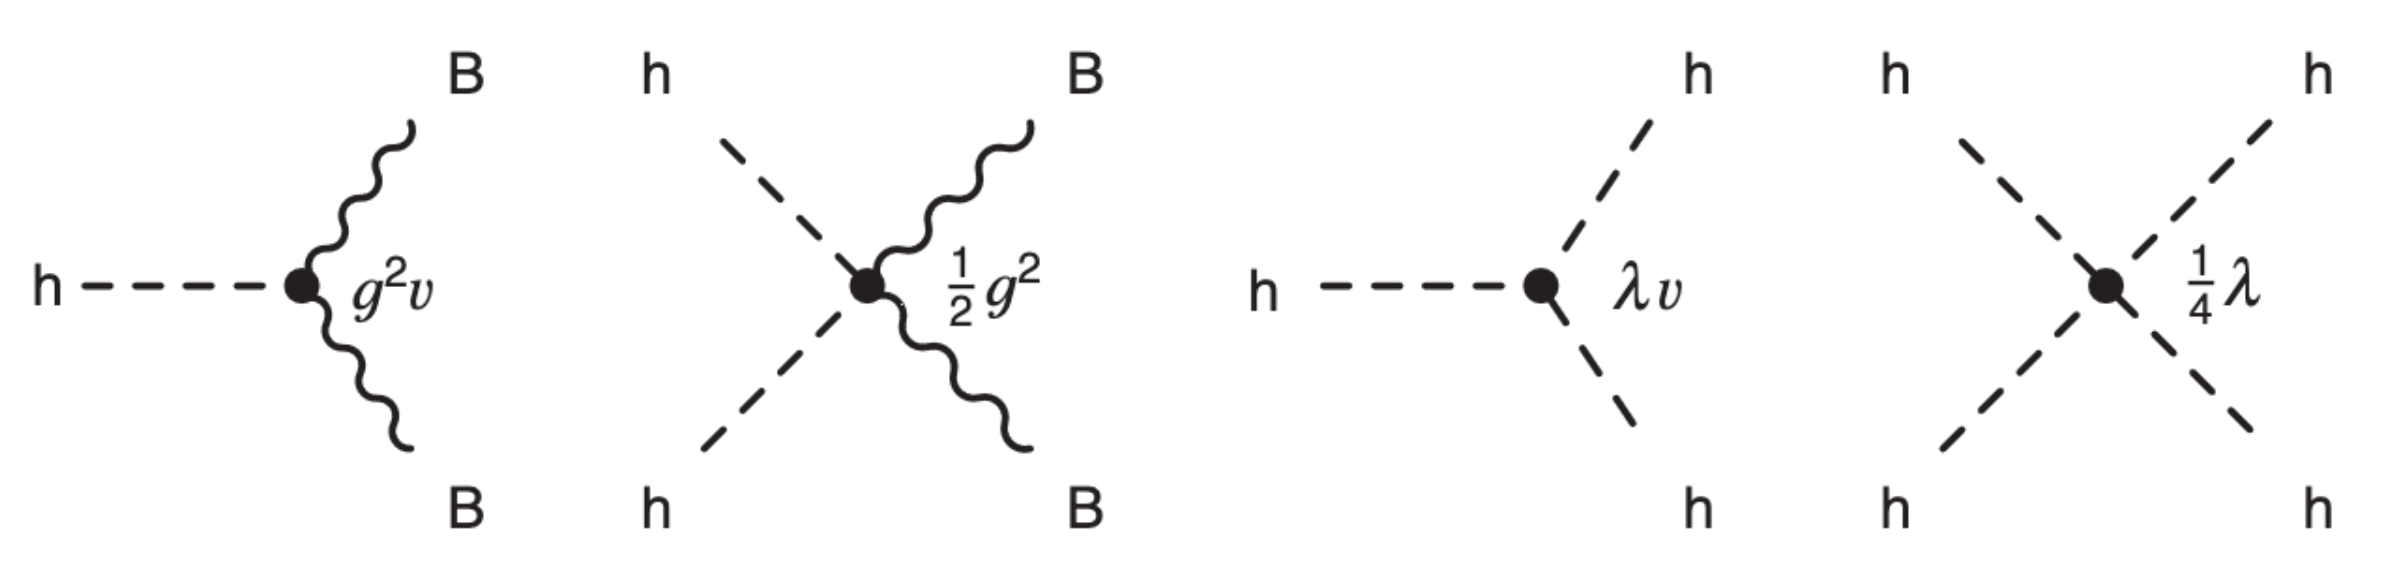
\includegraphics[width=.8\textwidth]{higgs_couplings}
    \caption[]{Higgs self interactions for a local $U(1)$ gauge symmetry. Adopted from \citep{thomson2013modern}.}
    \label{fig:higgs_couplings}
\end{figure}

\subsection*{The Standard Model Higgs}
For the electroweak Lagrangian the $SU(2)_L \otimes U(1)_Y$ symmetry is broken by the Higgs mechanism while maintaining the electromagnetic $U(1)_{EM}$ symmetry. This is also called \ac{ewsb} and is realized with a isospin doublet of complex scalar fields
\begin{equation}
    \phi(x)=
    \begin{pmatrix}
        \phi^+(x) \\
        \phi^0(x)
    \end{pmatrix}
    =
    \begin{pmatrix}
        \phi_1 (x)+i \phi_2 (x) \\
        \phi_3 (x)+i \phi_4 (x)
    \end{pmatrix}.
\end{equation}
with weak hyperchage $Y=1$. The upper state $\phi^+$ with $I_3=1/2$ is electrically charged and the lower state $\phi^0$ with $I_3=-1/2$ is electrically neutral consistent with the Gell-mann Nishijima formula from equation \ref{eq:gellmann_nishijima_formula}.


\subsubsection*{Higgs Term}
With $Y=1$ the covariant derivative from equation \ref{eq:cov_diff_L} becomes
\begin{equation}
    D_\mu=\partial_\mu- i g_2\frac{{\sigma}_a}{2}W_\mu^a+ ig_1\frac{1}{2}B_\mu.
\end{equation}
and the Higgs term for the electroweak Lagrangian of equation \ref{eq:L_EW} is
\begin{equation}
    \mathcal{L}_\text{Higgs}= \left(D_\mu\phi\right)^\dagger (D^\mu\phi)-V(\phi),
    \label{eq:L_higgs}
\end{equation}
with the Higgs potential
\begin{equation}
    V(\phi) = -\mu^2\phi^\dagger\phi+\frac{\lambda}{4}\left(\phi^\dagger\phi\right)^2.
    \label{eq:Higgs_initial_potential}
\end{equation}
In analogy to the steps for the $U(1)$ Higgs mechanism from section \ref{sec:higgs_mechanism} there is a set of degenerate minima for $\mu^2,\lambda>0$
\begin{equation}
    \phi^\dagger\phi=\frac{1}{2}(\phi_1^2+\phi_2^2+\phi_3^2+\phi_4^2)=\frac{v^2}{2}=\frac{4\mu^2}{\lambda}.
    \label{eq:higgs_vev}
\end{equation}
Since the photon needs to remain massless and as shown in section \ref{sec:higgs_mechanism} broken symmetries generate gauge bosons with mass, the \ac{vev} is chosen in a way that the vacuum shares the symmetry of the electromagnetic gauge group $U(1)_{EM}$ from section \ref{sec:qed} via setting \mbox{$\phi_1=\phi_2=\phi_4=0$} and $\phi_3=v$ such that the \ac{vev} becomes
\begin{equation}
    \langle0\vert \phi \vert0\rangle=\phi_0=\frac{1}{\sqrt{2}}
    \begin{pmatrix}
        0 \\
        v
    \end{pmatrix}.
\end{equation}
The generator of the electromagnetic subgroup is $Q=I_3+Y/2$. $\phi_0$ breaks $SU(2)_L$ and $U(1)_Y$ but since the lower state is electrically neutral $Q=0$, it remains locally gauge invariant under $U(1)_{EM}$ as can be seen from
\begin{equation}
    \phi_0 \rightarrow e^{i\alpha(x)Q}\phi_0=\phi_0.
\end{equation}
Expanding the field about the \ac{vev}
\begin{equation}
    \phi(x)=\frac{1}{\sqrt{2}}
    \begin{pmatrix}
        \phi_1 (x)+i \phi_2 (x) \\
        v+ \eta(x)+i \phi_4 (x)
    \end{pmatrix},
\end{equation}
becomes in the unitary gauge with the physical \ac{sm} Higgs field $h$
\begin{equation}
    \phi(x)=\frac{1}{\sqrt{2}}
    \begin{pmatrix}
        0 \\
        v+h(x)
    \end{pmatrix}.
    \label{eq:unitary_gauge}
\end{equation}
In this form the potential then becomes by virtue of equation \ref{eq:higgs_vev} in terms of $\mu$ and $v$
\begin{equation}
    V=\mu^2h^2+\frac{\mu^2}{v}h^3+\frac{\mu^2}{4v^2}h^4
    =
    \frac{m_h^2}{2}h^2+\frac{m_h^2}{2v}h^3+\frac{m_h^2}{8v^2}h^4.
    \label{eq:higgs_potential}
\end{equation}
This yields a Higgs mass term $m_h=\mu\sqrt{2}$ and triplet and quartic self-couplings proportional to the Higgs mass. The kinematic term of the Higgs Lagrangian can be brought into a form that the gauge fields $W^1_\mu,W^2_\mu,W^3_\mu,B_\mu$ represent the physical fields: the charged massive $W^{\pm}$ gauge bosons then are
\begin{equation}
    W_\mu^\pm = \frac{1}{\sqrt{2}}(W_\mu^1\mp i W_\mu^2),
\end{equation}
and the neutral massive $Z$ boson and the massless photon $A_\mu$ are mixed states of
\begin{equation}
    \begin{pmatrix}
        A_\mu \\
        Z_\mu
    \end{pmatrix}
    =
    \begin{pmatrix}
        \cos\theta_W  & \sin\theta_W \\
        -\sin\theta_W & \cos\theta_W
    \end{pmatrix}
    \begin{pmatrix}
        B_\mu \\
        W^3_\mu
    \end{pmatrix}
\end{equation}
rotated by the weak mixing angle $\theta_W$. The kinematic Higgs term then becomes
\begin{equation}
    \left(D_\mu\phi\right)^\dagger (D^\mu\phi )=
    \frac{1}{2}(\partial_\mu h)(\partial^\mu h)+
    \frac{g_2^2}{4}W^-_\mu W^{+\mu}(v+h)^2+
    \frac{g_1^2+g_2^2}{4} Z_\mu Z^\mu(v+h)^2.
    \label{eq:higgs_kinematic}
\end{equation}
% \begin{align}
%     \left(D_\mu\phi\right)^\dagger (D^\mu\phi )= &
%     \frac{1}{2}(\partial^\mu h)(\partial_\mu h)+
%     \frac{g_2^2}{4}W^-_\mu W^{+\mu}(v+h)^2+
%     \\
%                                                  & \frac{1}{2}\begin{pmatrix}
%                                                                   A_\mu & Z_\mu
%                                                               \end{pmatrix}
%     \begin{pmatrix}
%         m_A^2 & 0     \\
%         0     & m_Z^2
%     \end{pmatrix}
%     \begin{pmatrix}
%         A_\mu \\
%         Z_\mu
%     \end{pmatrix}
% \end{align}
and describes trilinear $HWW,HZZ$ and quadrilinear $HHWW,HHZZ$ vertices. The photon becomes naturally massless in this form and the masses of the massive gauge bosons can be read off
\begin{equation}
    m_W= \frac{1}{2}g_2v,\quad m_Z=\frac{1}{2}\sqrt{g_1^2+g_2^2}.
\end{equation}
Furthermore a relation to the weak mixing angle and the electric charge follow
\begin{equation}
    \cos\theta_W=\frac{g_2}{\sqrt{g_1^2+g_2^2}}=\frac{m_W}{m_Z}, \quad e=g\sin \theta_W.
\end{equation}
The $\cos\theta_W$ was verifiable before the Higgs discovery and a compelling argument for the Higgs to exist.

\subsubsection*{Yukawa Term}\label{sec:yukawa_term}
Fermion masses can be incorporated gauge invariant into the electroweak Lagrangian of equation \ref{eq:L_EW} with the help of the Higgs mechanism in the form of Yukawa couplings. For one generation of leptons and quarks gauge invariant terms are introduced via couplings between the left-handed doublet states, the Higgs field and right handed singlet states
\begin{align}
    \mathcal{L}_\mathrm{Y}^{\text{one gen}} & =
    - \; G_e
    \begin{pmatrix}
        \overline{\nu}_e & \overline{e} \\
    \end{pmatrix}_L
    \begin{pmatrix}
        \phi^+ \\
        \phi^0
    \end{pmatrix}
    e_R                                                                                                                                                                \\
                                            & \phantom{-\;}-G_d
    \begin{pmatrix}
        \overline{u} & \overline{d} \\
    \end{pmatrix}_L
    \begin{pmatrix}
        \phi^+ \\
        \phi^0
    \end{pmatrix}
    d_R                                                                                                                                                                \\
                                            & \phantom{-\;}-G_u
    \begin{pmatrix}
        \overline{u} & \overline{d} \\
    \end{pmatrix}_L
    \begin{pmatrix}
        \phi^{0*} \\
        -\phi^-
    \end{pmatrix}
    u_R                                                                                                                                                                \\
                                            & \phantom{-\;} +h.c.                                                                                                      \\
                                            & = -G_e \overline{L}_L \phi e_R -G_d \overline{Q}_L \phi d_R -G_u \overline{Q}_L \phi_c e_R + h.c. \label{eq:L_Y_one_gen}
\end{align}
with Yukawa coupling constant $G_e,G_d,G_u$ and the charge conjugated Higgs field $\phi_c=i\sigma_2\phi$. The latter can be used because it transforms just like the Higgs field and therefore leaves the Lagrangian gauge invariant. In the unitary gauge mass terms arise e.g. for the electron in the form
\begin{equation}
    \mathcal{L}_\mathrm{Y}^e=\frac{-G_e}{\sqrt{2}} v (\overline{e}_L e_R+\overline{e}_R e_L)+\frac{-G_e}{\sqrt{2}} h (\overline{e}_L e_R+\overline{e}_R e_L).
\end{equation}
The mass of a fermion $f$ is therefore
\begin{equation}
    m_f=G_f\frac{v}{\sqrt{2}},
\end{equation}
so that the full Yukawa Lagrangian can be written as
\begin{equation}
    \mathcal{L}_\mathrm{Yukawa}=-\sum_f m_f\overline{\psi}_f \psi_f -\sum_f \frac{m_f}{v}\overline{\psi}_f \psi_f h.
    \label{eq:yukawa_term}
\end{equation}
Consequently the Higgs couples to fermions proportional to their masses. In this form the spinors $\psi_f$ correspond to their mass eigenstates. Since physically observed states are mixed states of the mass eigenstates for the charged weak interactions, the formalism can be extended by making the Yukawa couplings $3\times 3$ matrices $G_u=G_{ij}^d$ with $i=u,c,t$ going over up type quarks and $j=d,s,b$ over down type quarks. Thus the quark part of the Yukawa Lagrangian of equation \ref{eq:L_Y_one_gen} becomes
\begin{equation}
    \mathcal{L}_\mathrm{Y}^{\text{quarks}} =
    -G_{ij}^d \overline{Q}_L^i \phi d_R^j -G_{ij}^u \overline{Q}_L^i \phi_c e_R^j + h.c.
\end{equation}
The $G_{ij}$ matrices mix the mass eigenstates and can be diagonalized with four unitary matrices $V_{L,R}^{u,d}$
\begin{equation}
    \Tilde{u}^i_{L,R}=(V^u_{L,R})_{ik}u^k_{L,R}, \quad \Tilde{d}^i_{L,R}=(V^d_{L,R})_{ik}u^k_{L,R}.
\end{equation}
With the identity $V_L^uV_L^{d\dagger}\equiv V_\mathrm{CKM}$ the quark mixing matrix also called \ac{ckm} matrix mixes the physical quark eigenstates
\begin{equation}
    \begin{pmatrix}
        d' \\
        s' \\
        b' \\
    \end{pmatrix}
    =V_\mathrm{CKM}\begin{pmatrix}
        d \\
        s \\
        b \\
    \end{pmatrix}=
    \begin{pmatrix}
        V_{ud} & V_{us} & V_{ub} \\
        V_{cd} & V_{cs} & V_{cb} \\
        V_{td} & V_{ts} & V_{tb} \\
    \end{pmatrix}
    \begin{pmatrix}
        d \\
        s \\
        b \\
    \end{pmatrix}.
\end{equation}
The $V_{ij}$ describes the transition probability for a quark $j$ to quark $i$ via the charged weak interactions. In this model neutrinos are assumed massless. Though they could be added including their mixing analogous to the quarks. This completes the current \ac{sm} electroweak Lagrangian of equation \ref{eq:L_EW}.

\section{Physics Beyond The Standard Model}\label{sec:beyond_sm}
The \ac{sm} works within its realm but is inherently incomplete and in discrepancy with other models. Most importantly there is no quantum theory for gravity excluding it entirely. The standard cosmological model - Lambda CDM - includes dark matter and dark energy to model the microwave background for which both the \ac{sm} offers no explanation. Furthermore neutrinos are known to be massive. In principle they can be added like fermions as in the section on the fermion Yukawa mass term \ref{sec:yukawa_term} but this requires right-handed neutrinos which have not been observed. This suggests, since their masses are much smaller than for the other fermions that there might be another mechanism responsible for the generation of the mass of neutrinos. Moreover, in the standard cosmological model, matter and antimatter should have been created in equal amounts, yet the universe is predominantly made of matter.

\begin{figure}
    \centering
    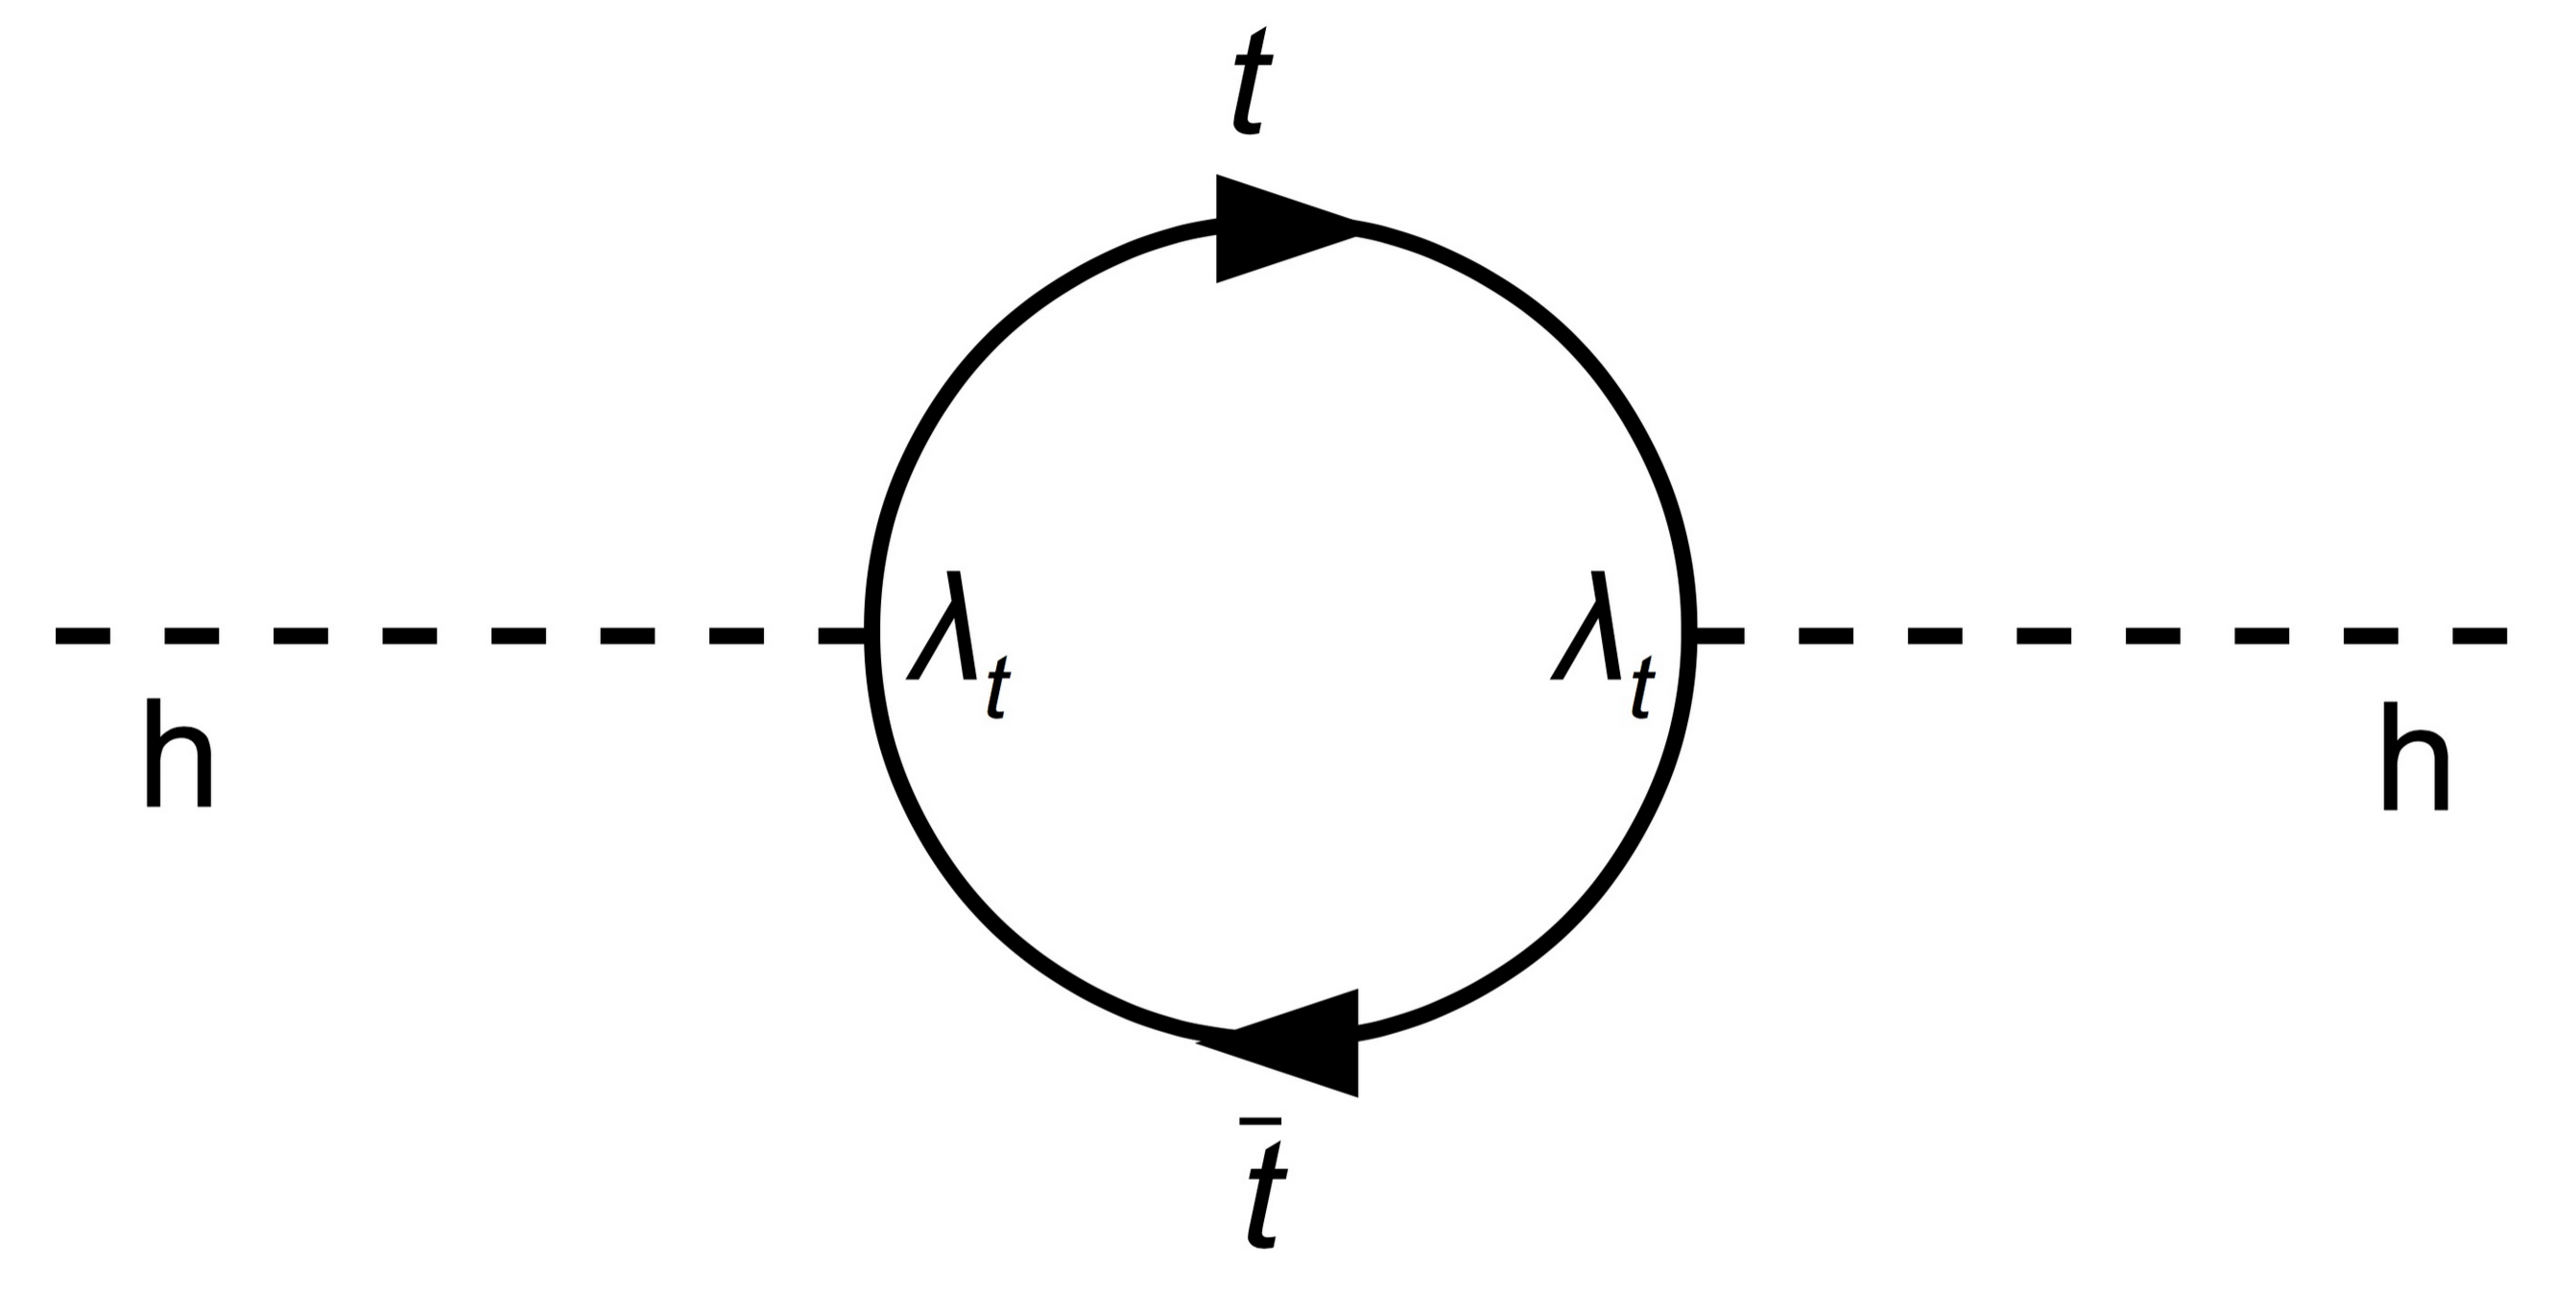
\includegraphics[width=0.35\textwidth]{top_loop}
    \caption[]{Leading correction to the Higgs field from top pair interaction.}
    \label{fig:top_loop}
\end{figure}
Especially with respect to the Higgs particle, it is not clear whether the assumed form of the Higgs potential is the one realized in nature since only the mass term of the Higgs potential from equation \ref{eq:higgs_potential} is determined by experiment. Considering top-quark loop corrections to the Higgs field, as illustrated in figure \ref{fig:top_loop}, the $\lambda(\mu)$ parameter in the Higgs potential becomes energy scale-dependent. At an instability energy scale of $\Lambda_I\approx \qty[]{e10}{GeV}$, $\lambda(\mu)$ could turn negative, suggesting that the current \ac{vev} might not be the absolute minimum of the Higgs potential but could be energetically lower or even unbounded. A phase transition via quantum tunneling into a different \ac{vev} could result in the universe's particles, forces and structures ceasing to exist and being replaced by different ones. The stability of the universe, under the assumptions of \ac{sm} physics, critically depends on the precise values of the Higgs and top quark masses, as depicted in the phase diagram in figure \ref{fig:vev_stability}, which places the universe at the boundary between stability and metastability given current measurement accuracies.

\begin{figure}
    \centering
    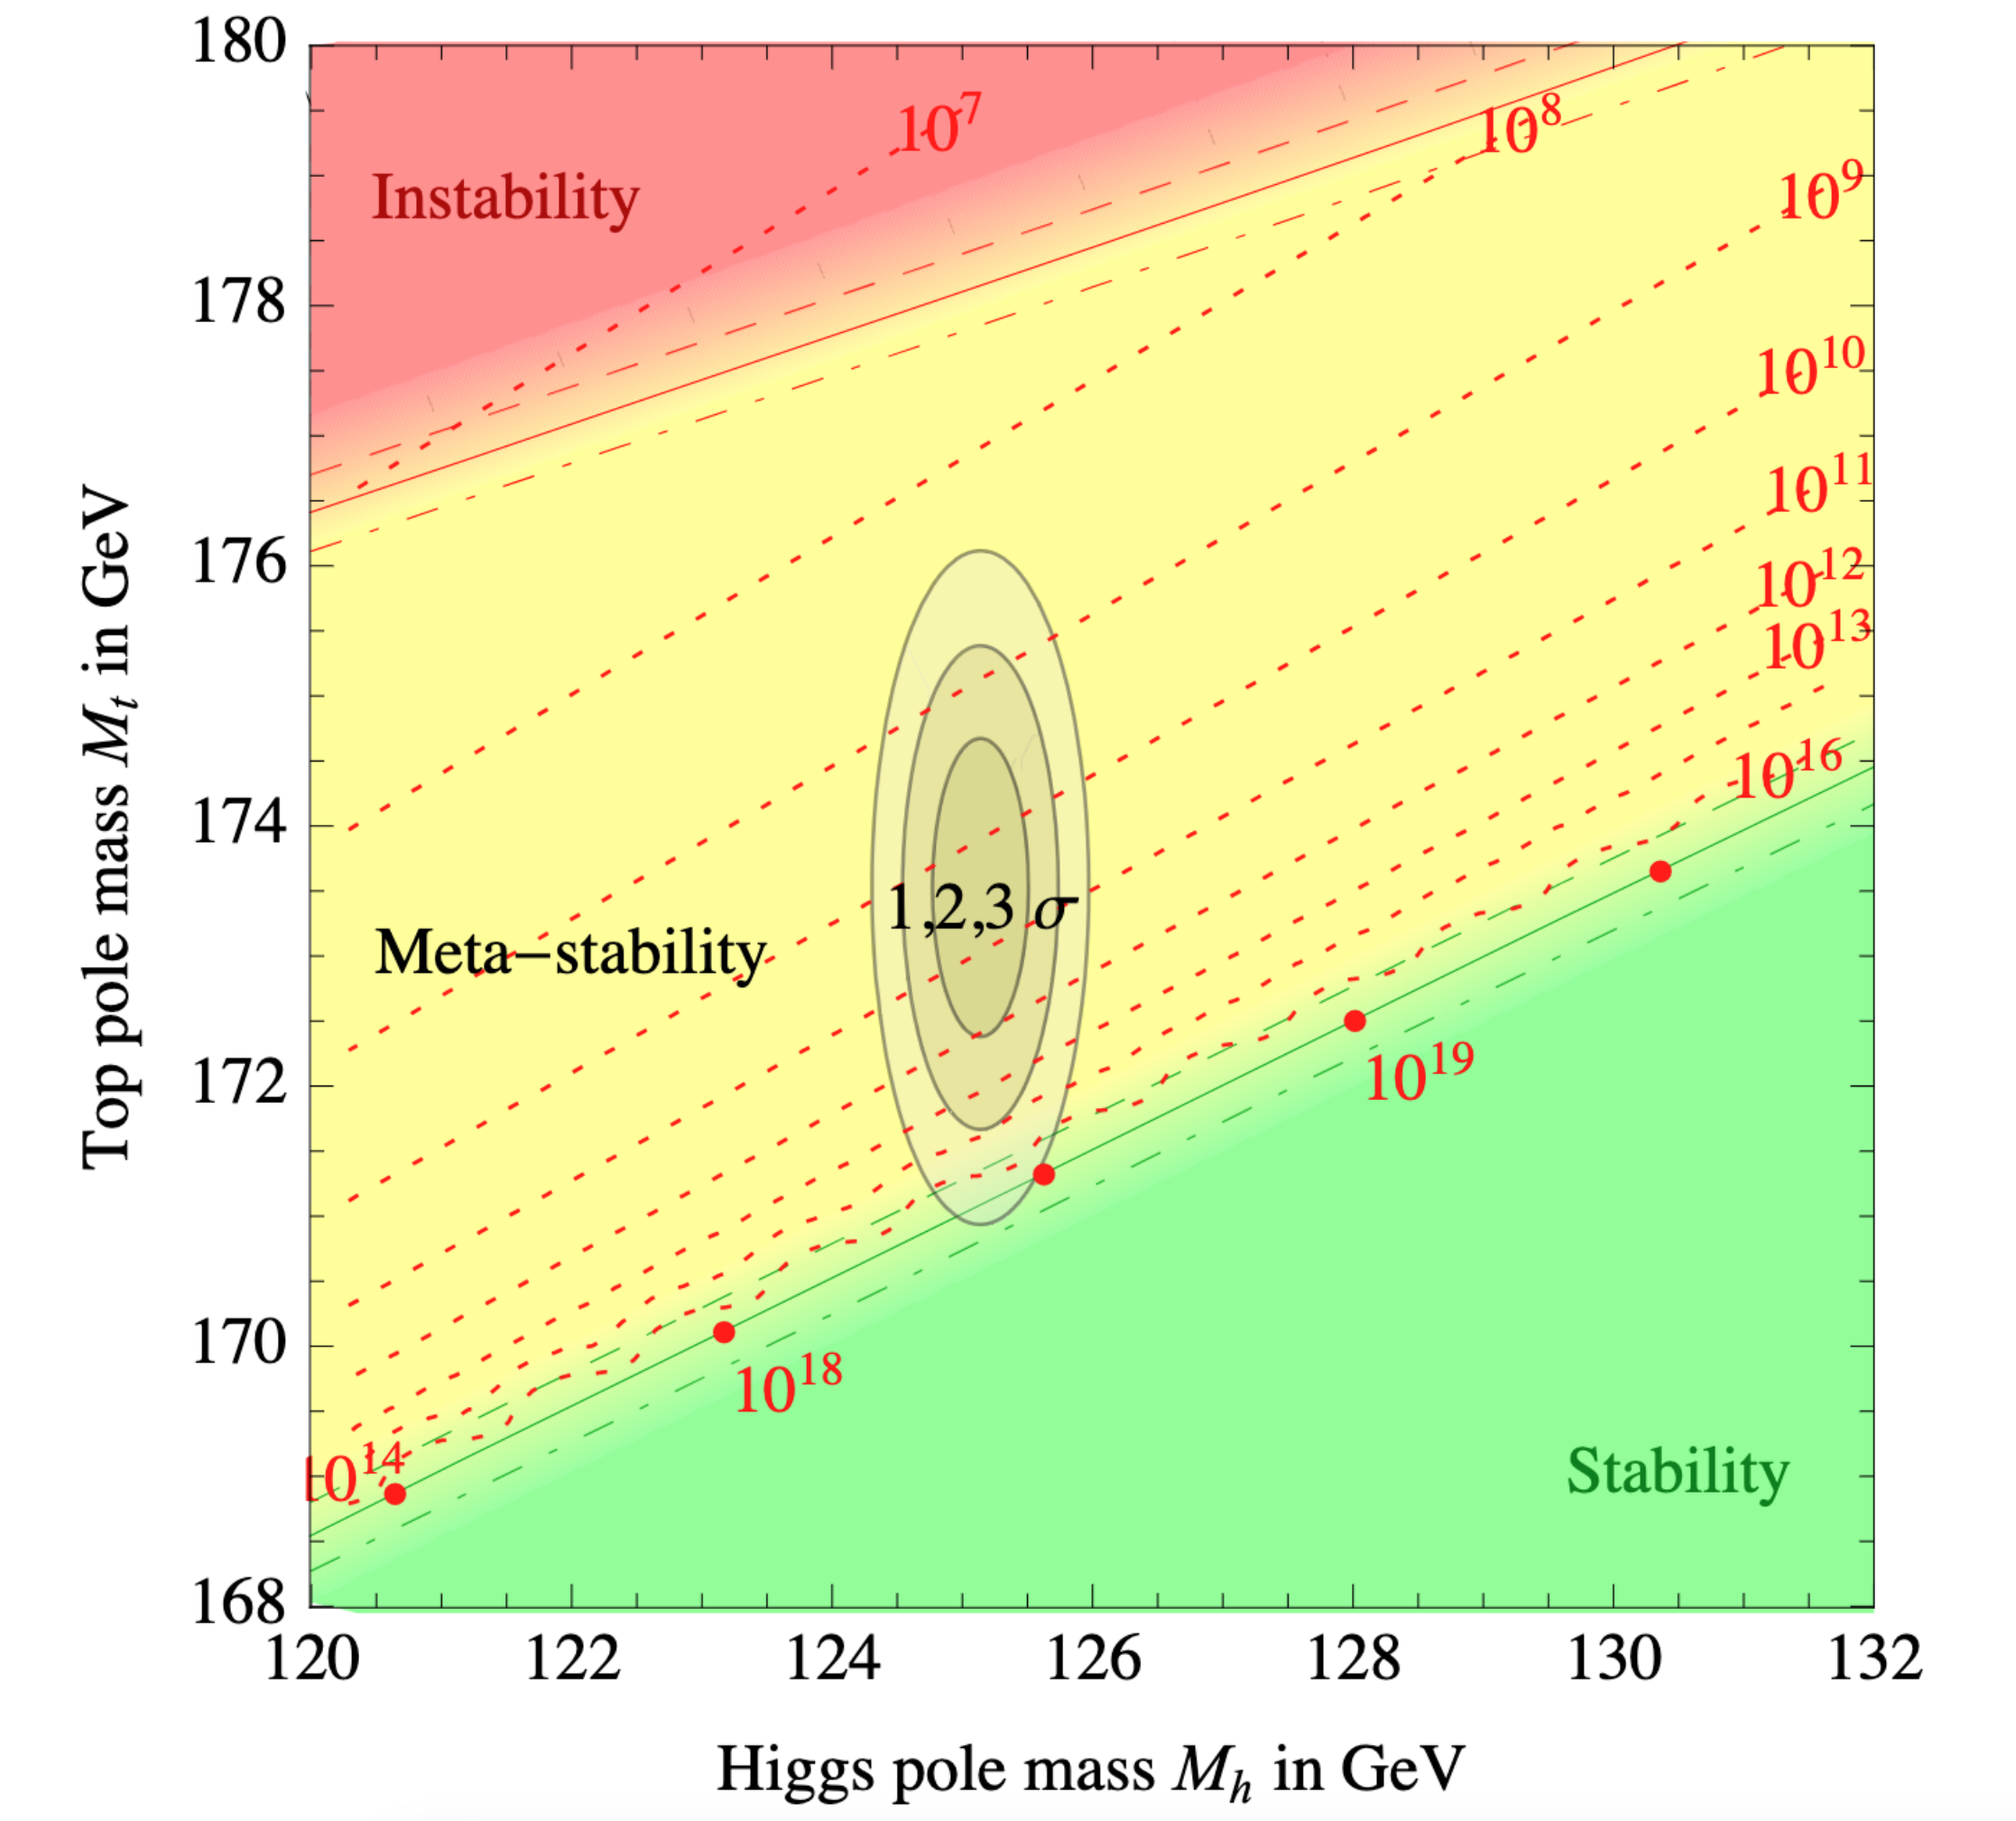
\includegraphics[width=0.7\textwidth]{vev_stability}
    \caption[]{Phase diagram of the stability of the universe assuming the \ac{sm} as a function of the Higgs and top pole masses. Instability for the Higgs potential occurs when due to quantum loop corrections the Higgs field develops a different minimum. Meta-stability is the case when there is an even lower global minimum in the potential and Stability means that there is only one global minimum. The red isolines correspond to the energy scale $\Lambda_I$ at which the Higgs potential becomes unstable. Adopted from \citep{Buttazzo:2013uya}.}
    \label{fig:vev_stability}
\end{figure}

Through the Higgs mechanism, elementary particles gain mass by interacting with the Higgs field. Accurate measurements of properties such as the mass and decay channels of the Higgs boson and the top quark offer means to validate and challenge the \ac{sm}. A precise understanding of these is crucial as any deviation from the expected values could indicate new physics. Moreover, the stability of our universe might be related to these properties. The study of the Higgs potential is therefore a promising endeavor to which this work aims to contribute.
